\documentclass{sprz}
\usepackage[backend=bibtex,style=numeric,sorting=none]{biblatex}
\usepackage{enumitem}

\addbibresource{bibliography.bib}

\studfield{Informatyka}
\studtype{Zaoczne}
\title{BatMonit -- system wykrywania nietoperzy na farmach wiatrowych}
\engtitle{BatMonit -- bat detection system on wind farms}
\acronym{Batmonit}
\titledate{2021-11-07}
\supervisor{dr Puźniakowski Tadeusz}
\author{Juliusz Orłowski}{s19799}{Aplikacje Internetowe}{Niestacjonarny}
\author{Jakub Prucnal}{s19800}{Sztuczna Inteligencja}{Niestacjonarny}
\author{Magdalena Wybraniec}{s19798}{Sztuczna Inteligencja}{Niestacjonarny}
\consultant{Dawid Gradolewski}
\consultant{Damian Dziak}
\projectgoals{Projekt typu R\&D, ma na celu przygotowanie systemu składającego się z dostępnego na rynku mikrofonu ultradźwięków odpowiedniego do zastosowania na turbinie wiatrowej oraz wytworzenienie oprogramowania pobierającego i analizującego dźwięk 
pochodzący z mikrofonu oraz rozpoznającego pojawienie się nietoperzy, zapisujący nagrania w bazie danych i wizualizujący je w interfejsie - panelu administratora. Dodatkowo celem będzie przygotowanie analizy odległości i kątów z jakiej mikrofon rejestruje głos nietoperzy i adekwatnie – zaproponowanie liczby i rozstawienia urządzeń nasłuchowych, tak aby pokryć kąt 360 stopni wokół turbiny na farmie wiatrowej.}
\productsandservices{System rejestrujący i wykrywający nietoperze z nagrań ultradźwięków, możliwy do połączenia z systemem wyłączania turbiny}
\mainfunctionalities{
\begin{itemize}
\item{Mikrofon ultradźwiękowy wraz z oprogramowaniem nagrywającym dźwięk}
\item{Urządzenie, do którego nagrania są przesyłane i w którym są przechowywane oraz automatycznie analizowane w poszukiwaniu na nim nietoperza}
\item{Baza danych, do której trafiają przeanalizowane nagrania}
\item{Interfejs wizualizujący nagrania}
\end{itemize}
}
\successmeasure{Oprogramowanie wykrywające i rozpoznające pojawienie się nietoperzy oraz wytworzenie lub dobranie z dostępnych na rynku urządzenia do rejestracji ultradźwięków. Dokonana analiza ulokowania urządzeń rejestrujących na wiatraku oraz jej akceptacja przez konsultanta z firmy Bioseco.}
\projlimitations{
Czas trwania projektu jest ograniczony do momentu przekazania książki dyplomowej do dziekanatu uczelni PJATK. Ograniczona dostępność nagrań głosów nietoperzy typu full-spectrum – możliwa sytuacja gdy tworzenie projektu będzie odbywało się na podstawie nagrań przetworzonych. Aktywność nietoperzy ma miejsce od końca marca do października – w związku z tym brak możliwości nagrywania ich aktywności w trakcie semestru zimowego – a tym samym brak możliwości wykonania prób hardware’u przed kwietniem 2024.
}
\date{\today}
\nabstract{TODO}




\begin{document}
\renewcommand{\labelenumii}{\arabic{enumi}.\arabic{enumii}}

\maketitle

\makeprojectcard
\makedeclaration

\tableofcontents

\chapter{Wstęp}\label{ch:wstep}

U podłoża rozwoju alternatywnych źródeł elektryczności leży uczynienie branży energetycznej bardziej „zieloną”, aby życie przyszłych pokoleń było przynajmniej tak samo dobre, jak nasze jest dzisiaj. W poszukiwaniu rozwiązań, które zabezpieczają społeczności w dobie globalnego 
ocieplenia,  zrównoważony rozwój stał się rdzeniem idei alternatywnych źródeł energii. Druga 
część historii posiada jednak swą ciemną stronę – wiele danych naukowych wskazuje na znaczący 
niekorzystny wpływ farm wiatrowych na przyrodę, a zwłaszcza nietoperze \cite{Wytyczne}. A są one ważnym elementem bioróżnorodności i poszukiwanego zrównoważonego rozwoju. Autorzy pracy dyplomowej w kooperacji z firmą Bioseco wypracowali oparty o sztuczną inteligencję system, który w przypadku dalszego jego rozwijania, zmniejszy śmiertelność nietoperzy na farmach wiatrowych i pomoże utrzymać branży wiatrowej miano ekologicznej. Chiropterologom zaś oraz urzędnikom oceniającym projekty wiatrowe pod kątem realizacji przyrodniczych norm prawnych, zapewni dodatkowe narzędzia minimalizacji wpływu farm na nietoperze.

\section{Cele projektu}

W ramach sformułowanego tematu wyszczególniono następujące cele badawcze i programistyczne:

\begin{itemize}
  \item{realizację działającego produktu o minimalnym zestawie funkcjonalności (ang: Minimal Viable Product, dalej: MVP) rejestrującego i wykrywającego nietoperze oraz wysyłającego sygnał wyłączenia – docelowo do systemu turbiny wiatrowej – składającego się z części sprzętowej i oprogramowania: aplikacji użytkwnika i bazy danych oraz modelu konwolucyjnych sieci neuronowych (ang: convoluted neural network, dalej CNN) oraz z aplikacji użytkownika i bazy danych,}
  \item{opracowanie koncepcji liczby i układu mikrofonów ultradźwięków docelowego produktu poprzez przeprowadzenie badań terenowych w zakresie zasięgu pracy testowanego sprzętu, tak by cały system pokrywał obszar 360 stopni dookoła turbiny wiatrowej, w odległości do około 100 m,}
  \item{opracowanie modelu sieci neuronowych uzyskującego przynajmniej 75\% skuteczności w identyfikacji nietoperzy - borowca wielkiego Nyctalus noctula i karlików Pipistrellus sp., głównych ofiar kolizji z turbinami wiatrowymi,}
  \item{przyczynienie się do rozwiązania realnego problemu występującego w obszarze branży energetyki wiatrowej oraz ochrony przyrody,}
  \item{rozpoczęcie współpracy z Bioseco Sp. z o.o. w celu zaprezentowania umiejętności studentów firmie oraz ich szybszego rozwijania dzięki kontaktowi z realnymi problemami biznesowymi, merytorycznymi, produkcyjnymi i wdrożeniowymi, rozwiązywanymi aktualnie przed doświadczony zespół specjalistów firmy.}
  \end{itemize}
  

\chapter{Podłoże projektu}

\section{Geneza problemu}

Lądowe farmy wiatrowe mogą mieć znaczący wpływ na środowisko naturalne, w szczególności na nietoperze \cite{Wytyczne}. Wszystkie gatunki nietoperzy w Polsce są objęte ścisłą ochroną gatunkową i podlegają ochronie prawnej zgodnie z Rozporządzeniem Ministra Środowiska z dnia 16 grudnia 2016 r. w sprawie ochrony gatunkowej zwierząt \cite{Rozporządzenie}. Tym samym inwestor realizujący inwestycję wiatrową przestrzegając prawa ochrony przyrody jest zobligowany uzyskać tzw. Decyzję Środowiskową (dalej: DŚ). Zawarte są w niej 
wszelkie informacje dotyczące: chiropterofauny danego obszaru, szacowanego wpływu inwestycji na nietoperze, działań zapobiegających i minimalizujących ewentualny wpływ inwestycji na nietoperze, tak by spełniała ona założenia dobrych praktyk i przepisy prawa – polskiego 
i międzynarodowego. 

Dotychczas przyjętą praktyką w przypadku wykrycia zbyt dużych aktywności nietoperzy w monitoringu rzedrealizacyjnym było wpisanie do DŚ obowiązkowych wyłączeń turbin w okresach, w których te zbyt duże aktywności wykryto \cite{Wytyczne}. Dzieje się tak między innymi dlatego, że nie istniał wcześniej system wykrywający nietoperze w czasie rzeczywistym, w którym akcja, taka jak wyłączenie turbiny mogła być podjęta o bieżące aktywności nietoperzy, warunki pogodowe i inne. Tymczasem dynamika użytkowania przestrzeni przez nietoperze jest bardzo zmienna w czasie i po realizacji inwestycji ssaki te w całych wyznaczonych okresach nie muszą być zagrożone. A wyłączenia turbin na długie okresy w roku wiążą się z ogromnymi stratami inwestorów. System zaproponowany w ramach niniejszej pracy inżynierskiej może przyczynić się do wspierania rozwoju nowych standardów na poziomie krajowym, europejskim i światowym, w zakresie niezbędnych działań minimalizujących wpływ farm wiatrowych na nietoperze. Zamiast dotychczas stosowanych, z góry określonych wyłączeń na długi okres przy określonej prędkości wiatru, mogłyby być wykorzystywane wyłączenia sterowane na bieżąco przez system – turbiny 
zatrzymywane byłyby tylko w czasie, kiedy większe liczebności nietoperzy 
faktycznie się pojawiają.

\section{Aktualne rozwiązania konkurencyjne}

Intensywny rozwój sieci neuronowych oraz internetu rzeczy (ang: IoT) przyczynił się do powstania podobnych rozwiązań. Na rynku światowym istnieją zbliżone pod kątem funkcjonalnym systemy, takie jak: DTBat i Fleximouse.

\section{IoT}

Mimo, że brak jest jednej definicji tego terminu, 
i w części publikacji nacisk kładziony jest na różne elementy tego 
paradygmatu \cite{iot-gov}, bardzo dobrej definicji dostarcza Kavin Ashton, 
uważany z ojca sformułowania "Internet of Things". Jest to "otwarta i 
kompleksowa sieć inteligentnych obiektów, które mają zdolność do 
samoorganizacji, udostępniania 
informacji, danych i zasobów, reagowania i działania w obliczu sytuacji
i zmian w otoczeniu" \cite{Ashton2002}. Definicję tę można uzupełnić tą 
sformułowaną przez IEEE jako sieć elementów - każdy wyposażony w czujniki - 
które są podłączone do internetu \cite{IEEE-iot}.

\section{Sieci neuronowe i uczenie głębokie}
Obecnie sieci neuronowe są bardzo ważną częścią świata nowoczesnych 
technologii i znajdują liczne zastosowania w obszarach autoamatyzujących 
wiele procesów takich jak analiza i diagnostyka medyczna \cite{diabetes}, 
wykrywanie oszustw finansowych \cite{laundring}, rekomendacje sprzedażowe 
\cite{fashion}, sterowanie procesów przemysłowych \cite{irigation} i wiele innych.

Uczenie głębokie jest podzbiorem sztucznej inteligencji. W procesie uczenia
głębokiego posiadając zbiór z odpowiednio zidentyfikowanymi elementami wykonujemy
serię nieliniowych przekształceń, tak aby otrzymana funkcja rozdzieliła zbiór 
niezidentyfikowanych elementów w taki sposób, by w każdej kategorii znalazły się 
tylko elementy danej klasy.

Struktura matematyczno-programistyczna, służąca do wytworzenia funkcji
klasyfikującej elementy zbioru, to właśnie sieć neuronowa. Zamysł konstrukcji
sieci neuronowej został zainspirowany budową ludzkiego mózgu. Składa się ona
z połączonych ze sobą warstw wielu neuronów. Każdy neuron składa się z 
wartości początkowej, wagi i funkcji aktywacji, wszystkie te wartości są 
wartościami matematycznymi. 

\begin{figure}[h]
  \centering
  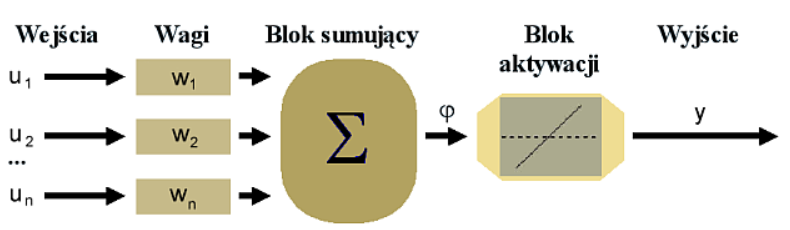
\includegraphics[width=0.8\textwidth]{sprz/neuron}
  \caption{Model neuronu. Źródło: \cite{neuron}}
  \label{img:neuron}
\end{figure} 

\section{Kooperacja z Bioseco S.A.}
Bioseco S.A. jest innowacyjną polską firmą technologiczną z siedzibą w Gdańsku, która opracowała systemy wizyjne wykorzystujące sztuczną inteligencję do ochrony zwierząt, głównie ptaków, na farmach wiatrowych i lotniskach. System opracowany i rozwijany jest w kierunku maksymalizacji ochrony zwierząt i minimalizacji strat produkcji. W związku z tym, że aktualnie większość klientów stanowią operatorzy farm wiatrowych, a obok problemu śmiertelności ptaków, drugim najważniejszym przyrodniczym problemem jest śmiertelność nietoperzy, w planach firmy znalazła się również eksploracja tego tematu i możliwość rozwoju technologii do ochrony nietoperzy. Jedna z osób z zespołu inżynierskiego posiada już wiedzę dziedzinową z zakresu zainteresowań Bioseco S.A. Po pomyślnych konsultacjach z firmą przygotowano temat i zakres współpracy spełniający wymogi pracy dyplomowej a jednocześnie zakres zainteresowań przedsiębiorcy.

\chapter{Metody pracy}

\section{Proces wytwórczy}

\subsection{Przyjęte podejście}
Zastosowano podejście hybrydowe: Water-Scrum-Fall. Prace rozpoczęto od przygotowania wymagań systemowych, analiz i wstępnego projektu systemu. W kolejnej fazie wytwarzania oprogramowania zastosowano metodę programowania zwinnego w oparciu o plany i dokumentację z pierwszego etapu, korygowane na bieżąco przy każdej itereacji. W ostateniej fazie, po zakończeniu etapu zwinnego, przewidziano testy systemowe i integracyjne.

\subsection{Organizacja zespołu}
Grupa inżynierska była samoorganizującym się zespołem. Część funkcji była silniej przypisana do konkretnych członków grupy:
Juliusz Orłowski - Software Developer, Jakub Prucnal - AI Developer, Software Engineer, Magdalena Wybraniec - Product Owner, Project Manager, specjalista dziedzinowy. 

\subsection{Charakterystyka przyrostów}
TODO

\section{Środowisko technologiczne}

\subsection{Technologie}
Sprzęt wykorzystany do realizacji ostatecznego rozwiązania to system SMART firmy Wildlife Acoustics. Pozostałe najważniejsze sprzęty wykorzystane do realizacji projektu to głośnik ultradźwiękowy Pettersson L400 i laptop DELL G3.

Model sieci neuronowej napisany został w języku Python z wykorzysteniem bibliotek PyTorch i TorchAudio.

Baza danych została przygotowana w MySQL.

Interfejs użytkownika został napisany w języku JavaScript z uzyciem biblioteki ReactJS. Serwer aplikacji został napisany w technologii NodeJS. Użyto również szeregu bibliotek wspomagających tworzenie aplikacji, bazy danych i testów: Sequelize, Express, Jest, Supertest, Joi, Jsonwebtoken. 

\subsection{Infrastuktura techniczna}
Na infrastrukturę techniczną, która umożliwiła realizację kluczowych elementów projektu dyplomowego składały się:
\begin{itemize}
  \item{Internet,}
  \item{sieć lokalna LAN firmy Bioseco,}
  \item{sieć światłowodowa turbiny wiatrowej,}
  \item{sprzęt komputerowy prywatny i służbowy,}
  \item{przęt do rejestracji nietoperzy (mikrofony ultradźwięków oraz system SMART),}
  \item{przęt do odtwarzania głosów nietoperzy (głośnik ultradźwiękowy Pettersson L400),}
  \end{itemize}

\subsection{Infrastuktura komunikacyjna i dokumentacja}
Kominikacja w ramach projektu odbywała się pomiędzy następującymi jednostkami:
\begin{itemize}
  \item{w obrębie grupy,}
  \item{pomiędzy grupą i Promotorem,}
  \item{pomiędzy grupą i Konsultantami.}
  \end{itemize}

Komunikacja w obrębie grupy inżynierskiej oraz pomiędzy grupą i Konsultantami z Bioseco S.A. i pozostałymi specjalistami odbywała się z wykorzystaniem wielu mediów:
\begin{itemize}
  \item{osobiście - spotkania w ramach zajęć na Uczelni,}
  \item{osobiście - spotkania poza zajęciami na Uczelni,}
  \item{osobiście - spotkania w ramach konsultacji,}
  \item{osobiście - spotkania w ramach pracy w Bioseco S.A.,}
  \item{aplikację Teams,}
  \item{aplikację Zoom,}
  \item{aplikację ClickUp,}
  \item{grupę w aplikacji WhatssApp,}
  \item{mailowo poprzez maile uczelniane, prywatne i służbowe}
  \item{telefonicznie.}
  \end{itemize}

  Komunikacja pomiędzy grupą inżynierską a Promotorem odbywała się poprzez następujące media:
\begin{itemize}
  \item{osobiście - spotkania w ramach zajęć na Uczelni,}
  \item{aplikację Teams,}
  \item{mailowo poprzez maile uczelniane.}
  \end{itemize}

Dokumentacja prowadzona była w:
\begin{itemize}
  \item{repozytorium na GitHub,}
  \item{aplikacji Teams,}
  \item{aplikacji ClickUp.}
  \end{itemize}

\section{Analiza zagrożeń}

Do głównych zagrożeń projektu należą \textit{de facto} te związane z ograniczonymi zasobami czasowymi oraz wiedzą i doświadczeniem, gdyż wpływa to łatwość/trudność poradzenia sobie z pozostałymi zagrożeniami. Pozostają jeszcze zagrożenie losowe, które jeśli wystąpią mogą sprawić, że możliwość realizacji projektu zmieni się diametralnie.

\subsection{Wpływ na realizację projektu}
Wpływ zagrożeń opisanych w niniejszym dokumencie jest potencjalnie wysoki, dlatego że projekt jest rozbudowany, innowacyjny, i powstaje na studiach zaocznych, w związku z czym zespół projektowy obłożony jest znaczną ilością dodatkowych obowiązków pozaszkolnych, a także pozbawiony jest dużego doświadczenia w realizacji tego typu projektów.

\subsection{Rekomendacje i rozwiązania}
Podsumowaniem szczegółowych rekomendacji umieszczonych w rozdziale - Załączniki - są zwłaszcza konsultacje ze specjalistami w wybranych dziedzinach, pomoc ze strony Bioseco S.A. w szczególności w rozmowach partnerskich związanych z pozyskaniem nagrań nietoperzy oraz zapewnianiem nowego sprzętu do eksperymentów, ciągła weryfikacja wymagań na system, wzajemne wsparcie i wsparcie bliskich, techniki relaksacyjne, sport.

\chapter{Prace badawczo-rozwojowe - projektowanie}

\section{Konsultacje z Bioseco S.A.}
W ramach kooperacji z Bioseco S.A. przeprowadzono spotkania wspomagające zespół inżynierski w procesie wytwórczym, udostępniono większość niezbędnego sprzętu oraz wiedzę z zakresu prowadzenia badań ternowych i opracowania danych, wytwarzania oprogramowania i działania dedykowanych sprzętów. Zrealizowano konfigurację sieciową udostępnionego sprzętu, tak aby umżliwić zdalny dostęp do danych z mikrofonu ultradźwieków. Zainstalowano również testowo mikrofon ultradźwięków na turbinie wiatrowej.

\section{Konsultacje chiropterologiczne i detektorowe}
W początkowej fazie przygotowania projektu przeprowadzono konsultacje chiropterologiczne obejmujące: pozyskanie zidentyfikowanych nagrań nietoperzy, typu nagrań jakich nalezy użyć do uczenia głębokiego, rodzaju rejestratorów ultradźwięków jakie mogą być wykorzystane na turbinie wiatrowej w rozwiązaniu końcowym. Konsultacje te przeprowadzono z najlepszymi polskimi chiropterologami oraz polskim, niemieckim i amerykańskim wytwórcą detektorów. Chiropterolodzy, z którymi przeprowadzono kolsultacje to: Aneta Zapart, Konrad Bidziński i Joanna Furmankiewicz. Firmy wytwarzające detektory, z którymi prowadzono kosultacje to: Animal Sound Labs, EcoObs, Wildlife Acoustics.

\section{Mikrofon ultradźwięków spełniający wymogi końcowego produktu}
W procesie definiowania cech sprzętu jakie powinien posiadać mikrofon i rejestrator ultrdźwięków wyszczególniono następujące cechy:
  \begin{itemize}
    \item{możliwie najwyższa jakość rejestrowanych ultradźwięków,}
    \item{możliwie największa odległość rejestrowanych ultradźwięków,}
    \item{wodoodporność,}
    \item{możliwość sprzętowa do integracji ze sprzętem i oprogramowaniem umożliwiającym pobieranie danych w czasie rzeczywistym.}
  \end{itemize}

W początkowym okresie prac nad systemem nie istniał mikrofon spełniające wszystkie powyższe kryteria. W mikrofonie otrzymanym początkowo z Bioseco brakowało wodoodporności. W detektorze Batcorder firmy EcoObs i mikrofonie SMM-U2 Wildlife Acoustics brakowało bezpośredniej możliwości podłączenia do urządzenia typu Raspberry Pi i nieograniczonego dostępu do danych. Wykonano próby współpracy z Animal Sound Labs, podczas których używając dostępnych najlepszych mikrofonów posiadanych przez firmę oraz projektując odpowiednią drogę analogowo-cyfrową z możliwością połączenia przez USB do urządzenia typu Raspberry Pi miał powstać odpowiedni mikrofon, jednak próby te zakończyły się niepowodzeniem z uwagi na ograniczenia czasowe Animal Sound Labs w zaproponowanym terminie. W tym czasie na rynku pojawiło się nowe urządzenie firmy Wildlife Acoustics - system SMART, który dostarczył wszystkich niezbędnych elementów, jakie wymagane były od sprzętu do realizacji niniejszej pracy dyplomowej (\ref{img:smart}). 

\begin{figure}[h]
  \centering
  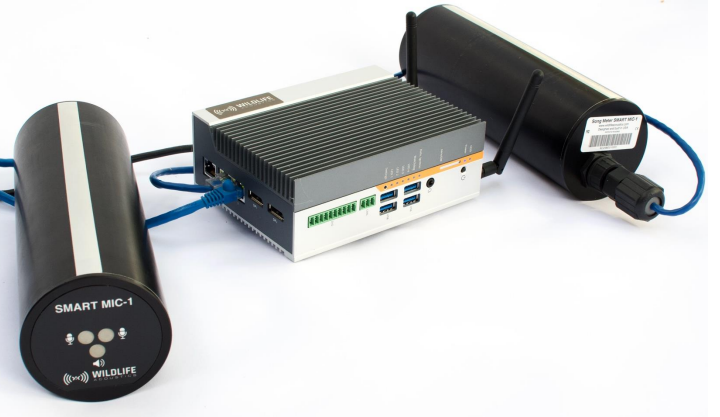
\includegraphics[width=0.8\textwidth]{sprz/smart.png}
  \caption{System SMART firmy Wildlife Acoustics. Źródło: Wildlife Acoustics}
  \label{img:smart}
\end{figure} 

Z korzyścią dla ochrony nietoperzy i deweloperów farm wiatrowych, a z pewnymi zagrożeniami dla twórców niniejszej pracy dyplomowej mikrofon został wyprodukowany wraz z tzw. kontrolerem (prostym przemysłowym koputerem), który wyposażony jest w oprogramowanie pobierające dane z mikrofonu i po odpowiedniej konfiguracji sieciowej serwujący dane i prezentujący je w interfejsie użytkownika. Mimo tego, że całe rozwiązanie częściowo odpowiada zakresowi niniejszej pracy dyplomowej, nie jest ono idealne, np. nie posiada bazy danych czy też w dość znacznym stopniu niepoprawnie identyfikuje gatunki nietoperzy. Mimo to, fakt pracy członków zespołu nad podobnym rozwiązaniem, z uwagi na obszerne zajęcie się takim tematem i wdrożenie się w wiele jego aspektów, niesie raczej możliwości i szanse rozwoju tego rozwiązania, niż zagrożenie ze strony konkurencji.

\section{Odtwarzanie ultradźwięków}
Do wyemitowania ultradźwięków niezbędne są urządzenia obsługujące co najmniej dwukrotnie wyższą częstotliwość niż emitowane dźwięki. Wynika to z twierdzenia Nyquista-Shannona, zgodnie z którym częstotliwość próbkowania z sygnału ciągłego ("analogowego") na dyskretny ("cyfrowy")musi być co najmniej dwukrotnie wyższa od najwyższej składowej widma sygnału aby sygnał został odtworzony poprawnie i nie dochodziło do zjawiska aliasingu \cite{probkowanie}. W zależności od możliwości karty dźwiękowej w komputerze użytym jako generator ultradźwięków, należy bądź ustawić maksymalną wartość próbkowania karty, bądź podłączyć wzmacniacz zwiększający maksymalną częstotliwość odtwarzania.

Do wstępnych testów poprawności działania sprzętu użyto wzmacniacza iFi Zen Dac o maksymalnej częstotliwości odtwarzania 384 kHz, a do testów terenowych mikrofonu - laptopa DELL G3 z maksymalną częstotliwością próbkowania karty dźwiękowej ustawioną na 96 kHz.

\section{Głosy nietoperzy typu full-spectrum}
Dźwięk typu full-spectrum, to rodzaj nagrania i analizy spektralnej dźwięku, w którym ujęte jest pełne spektrum nagrywanych częstotliwości. W odróżnieniu np. od nagrań typu zero-crossing posidają dużo więcej informacji o dźwięku, co przedstawiono na ilustracji (\ref{img:fullspectrum}). Z tego powodu nagrania takie są najlepsze do analizy gatunków nietoperzy, a wykorzystanie tego typu nagrań może dać najlepsze efekty w treningu sieci neuronowej oraz predykcji gatunków.

Tego typu nagrania generowane są tylko przez część detektorów ultradźwięków - tylko przez najnowocześniejsze rekordery, co wpłynęło na zmniejszenie liczby potencjalnych źródeł nagrań do treningu sieni neuronowej.

\begin{figure}[h]
  \centering
  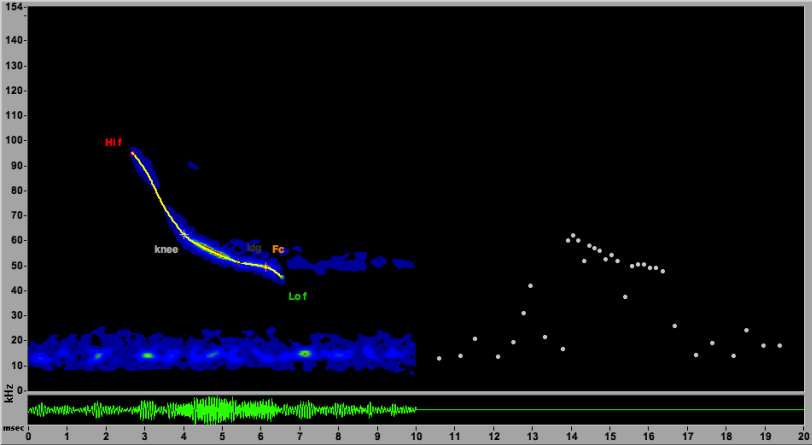
\includegraphics[width=0.8\textwidth]{sprz/fullspectrum.png}
  \caption{Porównanie dźwięku typu full-spectrum (po lewej) z dźwiękiem typu zero-crossing (po prawej). Źródło: \cite{fullspectrum}}
  \label{img:fullspectrum}
\end{figure} 

\subsection{Wytworzenie sztucznych głosów nietoprzy do wstępnych testów sprzętu}

W celu przetestowania działania sprzętu rejestrującego i oprogramowania przetwarzającego zarejestrowane dźwięki, przeprowadzono doświadczenie polegające na sztucznym wytworzeniu dźwięków, które imitowały by głos nietoperza.
Pierwszym etapem było wygenerowanie w programie Audacity sinusoidalnej fali dźwiękowej z początkową częstotliwością 51 kHz i końcową częstotliwością 42 kHz, amplitudą początkową 0 i amplitudą końcową 1, interpolacją logarytmiczną oraz czasem trwania 25 ms (\ref{img:wykres_fali}).

\begin{figure}[h]
    \centering
    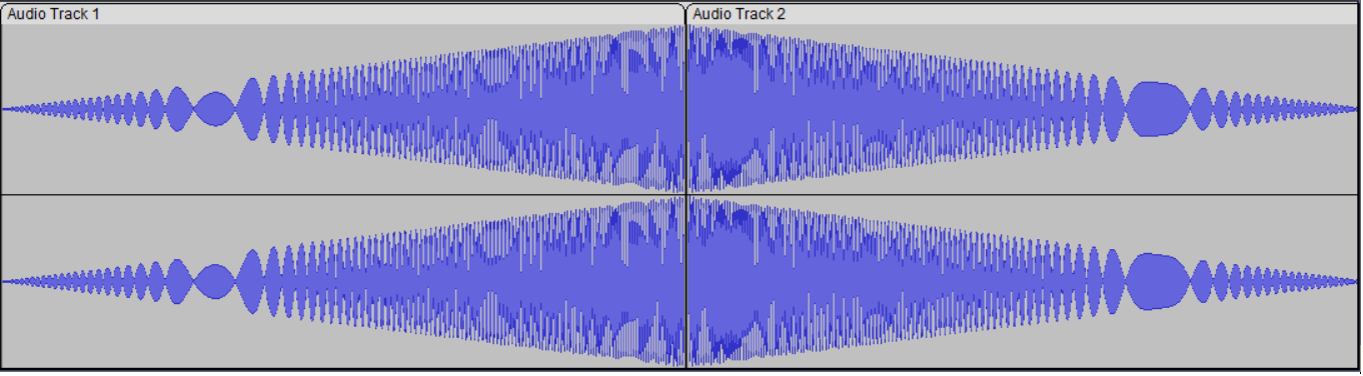
\includegraphics[width=0.8\textwidth]{sprz/wykres_fali}
    \caption{Wykres fali dźwiękowej}
    \label{img:wykres_fali}
\end{figure}

Uzyskany w ten sposób wykres fali dźwiękowej skopiowano dziesięciokrotnie i utworzono sekwencję 500 ms dźwięków, przed którą i po której wprowadzono 500 ms ciszy w celu łatwiejszego wyodrębnienia dźwięków po ich późniejszym zarejestrowaniu (\ref{img:wykres_fali_wielokrotnej}).

\begin{figure}[h]
    \centering
    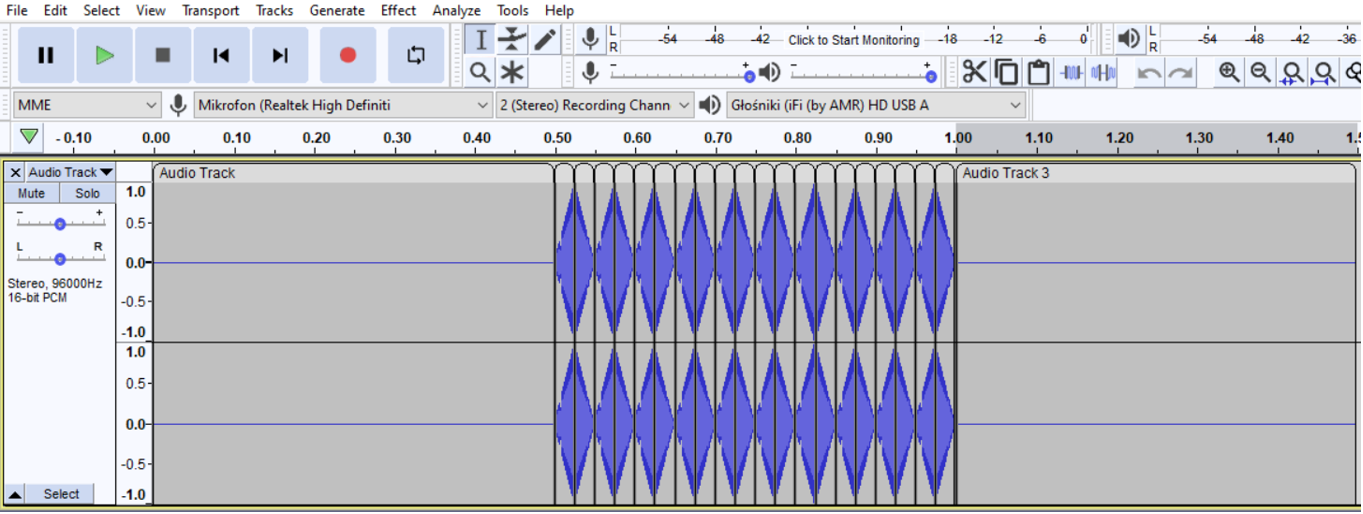
\includegraphics[width=0.8\textwidth]{sprz/wykres_fali_wielokrotnej}
    \caption{Zwielokrotniony wykres fali}
    \label{img:wykres_fali_wielokrotnej}
\end{figure}

Następnie, do wyemitowania dźwięku doświadczenia niezbędne były urządzenia obsługujące co najmniej dwukrotnie wyższą częstotliwość niż emitowane dźwięki. W tym celu do komputera służącego jako generator dźwięku podłączono wzmacniacz iFi Zen Dac o maksymalnej częstotliwości odtwarzania 384 kHz oraz głośnik ultradźwiękowy Pettersson L400 (10-110 kHz). Do zarejestrowania wyemitowanego dźwięku posłużył mikrofon Pettersson M500-384 o częstotliwości próbkowania 384 kHz.

Program BatSound dołączony do mikrofonu posłużył do wizualizacji zarejestrowanego dźwięku.

\begin{figure}[h]
    \centering
    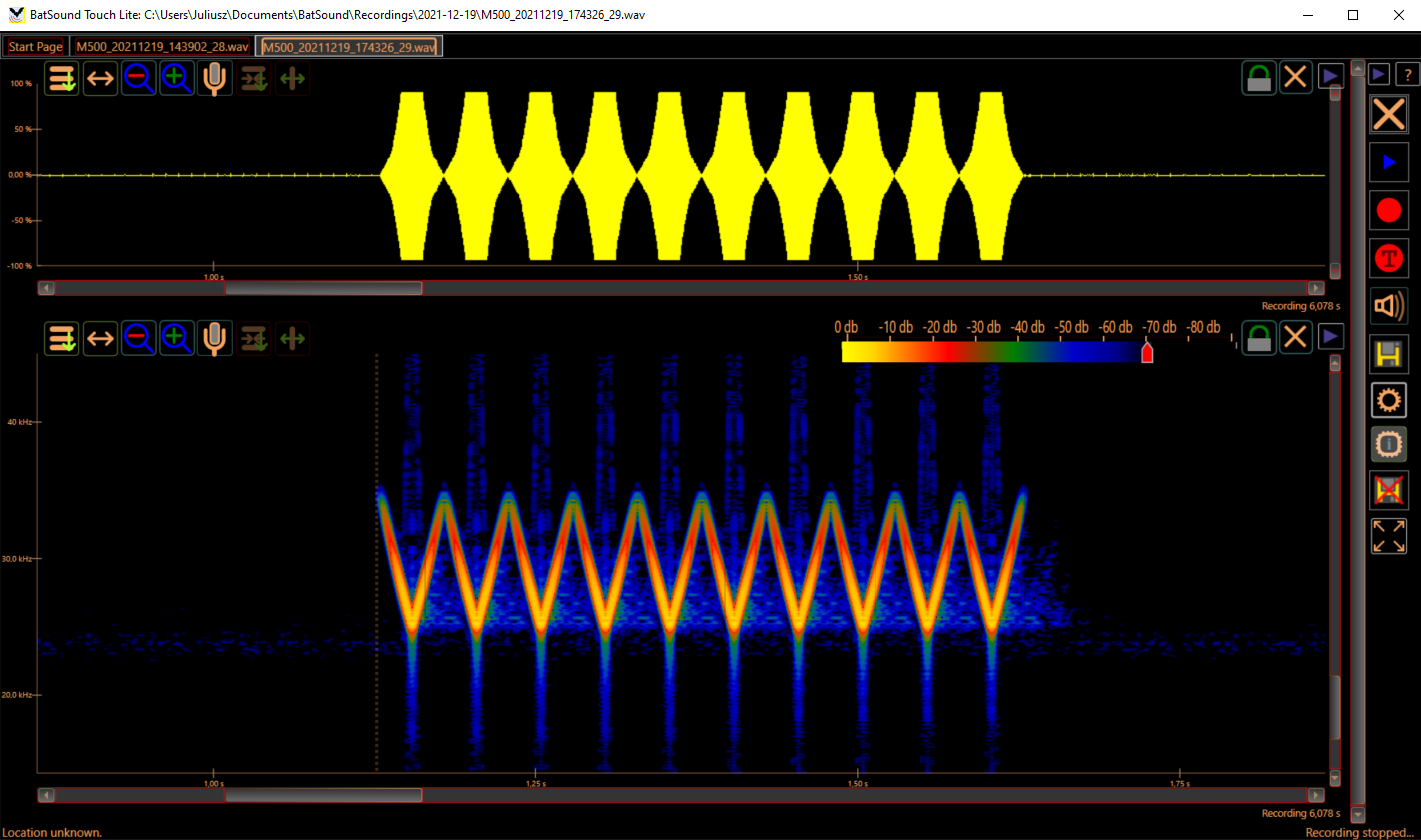
\includegraphics[width=0.8\textwidth]{sprz/batsound}
    \caption{Wykres zarejestrowanego dźwięku zwizualizowany w programie Batsound}
    \label{img:batsound}
\end{figure}

Powyższe doświadczenie dowiodło, iż mikrofon Pettersson M500-384 spełnia swoje zadanie. Mikrofon rejestruje dźwięki w zakresie niesłyszalnym dla człowieka i poprawnie wizualizuje zarejestrowane nagranie.

\subsection{Wytworzenie sztucznych głosów nietoprzy do testów terenowych mikrofonu}
W identyczny sposób jak głosy nietoprzy do wstępnych testów sprzętu przygotowano też dźwięki do testów terenowych. Dźwięki miały częstotliwości: 16-20 kHz, 25-35 kHz, 37-40 kHz i 40-48 kHz. Poszczególne dźwięki zostały zaprojektowane tak, aby reprezentować zakresy częstotliwości najczęściej występujących grup nietoperzy, a jednocześnie nie nakładały się na siebie – dzięki czemu można je było łatwo rozróżnić w wynikach. Poszczególne zakresy częstotliwości odpowiadają następującym gatunkom:

\begin{itemize}
  \item{16-20 kHz – borowiec, borowiaczek,}
  \item{25-35 kHz – mroczek posrebrzany, mroczek późny, mroczek pozłocisty i kilka gatunków z rodzaju Myotis,}
  \item{37-40 kHz – karlik większy i kilka gatunków z rodzaju Myotis}
  \item{40-48 kHz – karlik większy i karlik malutki.}
\end{itemize}

Większość z tych nietoperzy to gatunki szczególnie narażone na kolizje z turbinami wiatrowymi, to jest: borowiec, borowiaczek, karliki czy mroczek posrebrzany.

\subsection{Zebranie nagrań nietoperzy}
Zebranie nagrań nietoperzy odpowiedniego typu i odpowiedniej ich liczby rodziło kilka problemów:
\begin{itemize}
  \item{nagrania typu full-spectrum pochądzą z najnowoczesniejszych detektorów, które nie są używane przez wsystkich chiropterologów, więc ogranicza to grupę osób posiadających takie nagrania,}
  \item{nagrania powinny pochodzić ze środowiska podobnego do lokalizacji turbin wiatrowych, najlepiej z turbiny wiatrowej z uwagi na podobne składy gatunkowe nietoperzy jakie napotykane będę przez urzadzenie po wdrożeniu, a więc powinny pochodzić z monitoringu porealizacyjnego, który prowadzony jest w Polsce przez niewielką grupę chiropterologów, co zmniejsza liczbę osób posiadających takie nagrania}
  \item{nagrań musi być możliwie dużo, do celów skutecznego treningu sieci neuronowej}
  \item{kwestie związane z własnością, potencjalne koszty i związane z tym negocjacje.}
\end{itemize}

Po trwających kilka miesięcy poszukiwaniach osób mogących udostępnić takie nagrania, negocjacjach warunków przekazania nagrań oraz samym procesie przekazywania nagrań, udało się pozyskać 71,7 GB danych, w tym 18 412 nagrań zawierających odgłosy nietoperzy oraz inne dźwięki, takie jak szumy pochodzące z otoczenia.

\chapter{Prace badawczo-rozwojowe - testy terenowe}

\section{Montaż systemu SMART na turbinie wiatrowej}
System SMART firmy Wildlife Acoustics został zainstalowany na jednej z farm wiatrowych, na których operuje firma Bioseco S.A. przez pracowników firmy. Instalacja miała miejsce 14 lipca 2023 (\ref{img:smart-installed}). 

\begin{figure}[h]
  \centering
  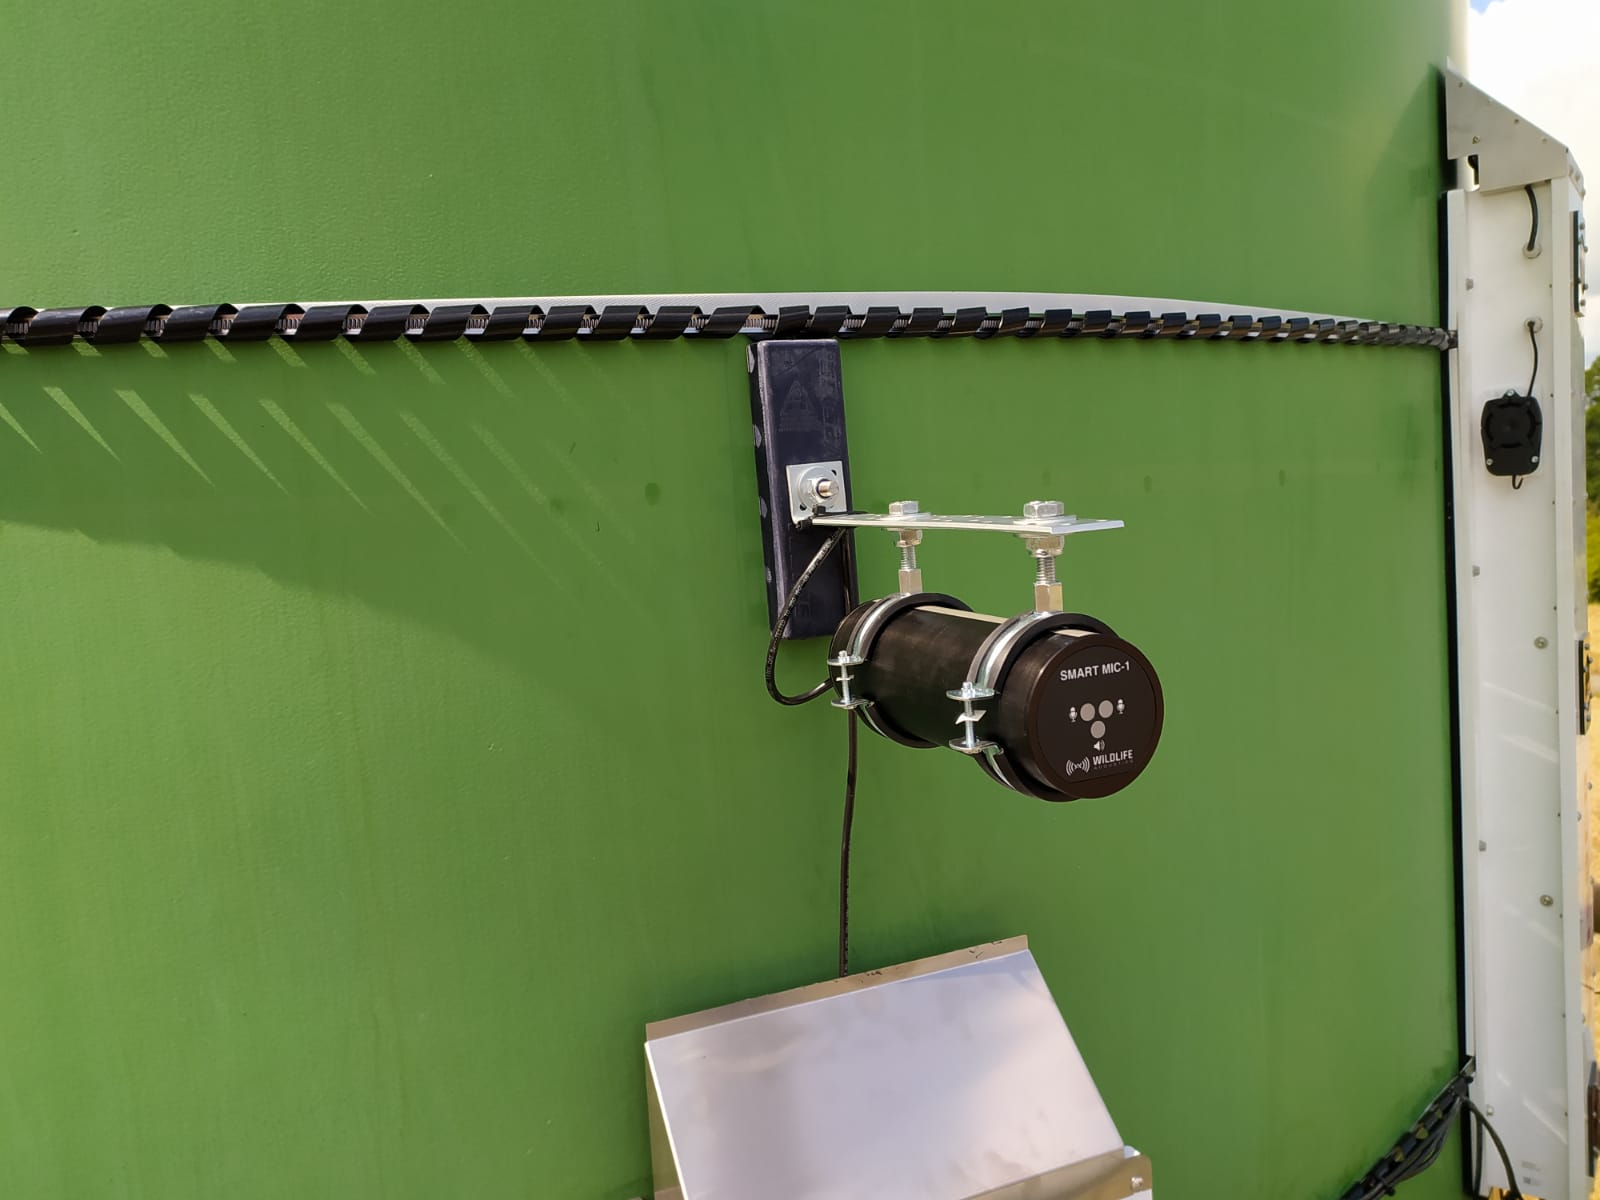
\includegraphics[width=0.8\textwidth]{sprz/smart-installed.png}
  \caption{System SMART firmy Wildlife Acoustics zainstalowany na turbinie wiatrowej. Źródło: Bioseco}
  \label{img:smart-installed}
\end{figure} 

\section{Konfiguracja sieciowa}
Konfiguracja sieciowa systemu SMART została zrezlizowana przez Bioseco. SMART został połączony poprzez Ethernet do skrzynki zasilająco-sieciowej Bioseco zainstalowanej w turbinie wiatrowej, poprzez którą system podłączony jest światłowodem do Internetu. Port sieciowy udostępniony z turbiny skonfigurowany jest w taki sposób, aby poprzez VPN w sieci Bioseco możliwy był dostęp do danych z mikrofonu.

\section{Konsultacje z Wildlife Acoustics}
Konsultacje z firmą Wildlife Acoustics obejmowały takie elementy jak:
\begin{itemize}
  \item{lokalizacja mikrofonu na turbinie wiatrowej (wieża/gondola),}
  \item{lokalizacja kontrolera na turbinie wiatrowej (wieża/gondola),}
  \item{liczba mikrofonów,}
  \item{sposób montażu.}
\end{itemize}

W celu poprawnego zaadresowania powyższych elementów należało uwzględnić następujące aspekty:

\begin{itemize}
  \item{wysokość przelotów nietoperzy, których dotyczy problem śmiertelności,}
  \item{możliwości technologiczne sprzętu, np. najdłuższa możliwa długość kabla Ethernet łączącego mikrofon z kontrolerem,}
  \item{możliwość wytwarzania echa przez elemeny turbiny bądź w wyniku nieprawidłowego montażu mikrofonu, co może powodować nieprawidłowości w rejestracji głosów nietoperzy,}
  \item{możliwość lokalizacji sprzętu w turbinie z punktu widzenia deweloperów farm wiatrowych, np. problem lokalizacji źródła zasilania w gondoli,}
  \item {możliwości technologiczne montażu w różnych częściach turbiny i problem dostępu do sprzętu w przypadku jego konserwacji czy naprawy,}
  \item {występowanie badź nie zaleceń władz środowiskowych co do szczegółów montażu podobnych urządzeń na farmach wiatrowych.}
\end{itemize}

Kluczowe ustalenia z konsultacji są następujące:
\begin{itemize}
  \item{lokalizacja mikrofonu na turbinie wiatrowej najlepiej jeśli będzie w gondoli, ale może być również u podstawy wieży,}
  \item{zaleca się stosowanie dwóch mikrofonów na jednej turbinie, ale możliwy jest montaż jednego mikrofonu, bądź większej ich liczby,}
  \item{z uwagi na ograniczenia w długości kabla Ethernet, który łączy mikrofon z kontrolerem (do 100 m) oraz fakt, że nowoczesne turbiny wiatrowe posiadają wieże wyższe niż 100 m, mikrofon razem z kontrolerem powinny znajdować się albo w gondoli albo na dole wieży turbiny,}
  \item{możliwy jest montaż poprzez umieszczenie mikrofonu w otworze wywierconym w gondoli bądź na szczycie gondoli zamocowany do zewnętrznych elementów gondoli.}
\end{itemize}

\section{Metodyka testów}
Sztucznie przygotowane dźwięki emitowano w kilku konfiguracjach, składających się z różnych odległości, kątów względem mikrofonu i częstotliwości. Dźwięki o częstotliwościach: 16-20 kHz, 25-35 kHz, 37-40 kHz i 40-48 kHz odtwarzane były w odległościach 7, 20, 40, 60, 80, 100 i 120 m od mikrofonu. Dźwięki odtwarzane były w czterech liniach przebiegających pod kątami 0, 30, 60 i 90 stopni w stosunku do przodu mikrofonu (\ref{img:angles}). Dźwięki odtwarzane były z zestawu głośnika ultradźwiękowego Pettersson L400 oraz laptopa z kartą dźwiękową w konfiguracji umożliwiającej odtwarzanie dźwięków o wysokiej częstotliwości (16-bit, 48 kHz). Dzwięki odtwarzane były w możliwie najwyższym natężeniu. Każdy dźwięk był emitowany w określonej odległości i pod określonym kątem od trzech do sześciu razy, w większości przypadków trzy razy.

\begin{figure}[h]
  \centering
  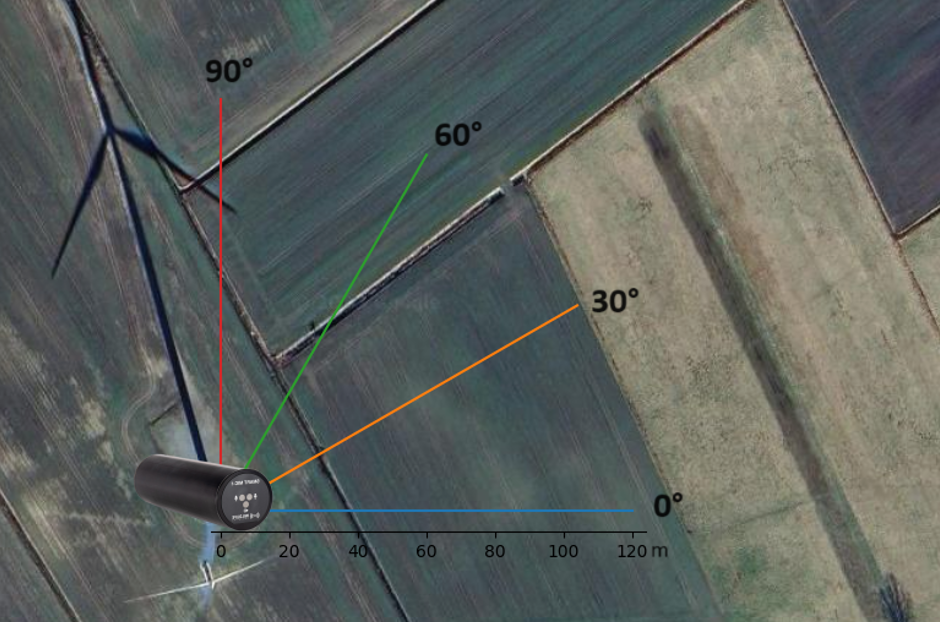
\includegraphics[width=0.8\textwidth]{sprz/angles.png}
  \caption{Zilustrowanie konfiguracji odległości i kątów od przodu mikrofonu, pod jakimi odtwarzane były dźwięki o poszczególnych częstotliwościach. Źródło: Google Maps}
  \label{img:angles}
\end{figure} 

\section{Realizacja testów w terenie}
Badania przeprowadzono w dniu 8 września 2023 roku zgodnie z przedstawioną powyżej metodyką w następujących warunkach atmosferycznych: 26 stopni C, zachmurzenie – 10\%, prędkość wiatru – 2-4 m/s, kierunek wiatru – NE, wilgotność – 40\% (\ref{img:fieldtests}).

\begin{figure}[h]
  \centering
  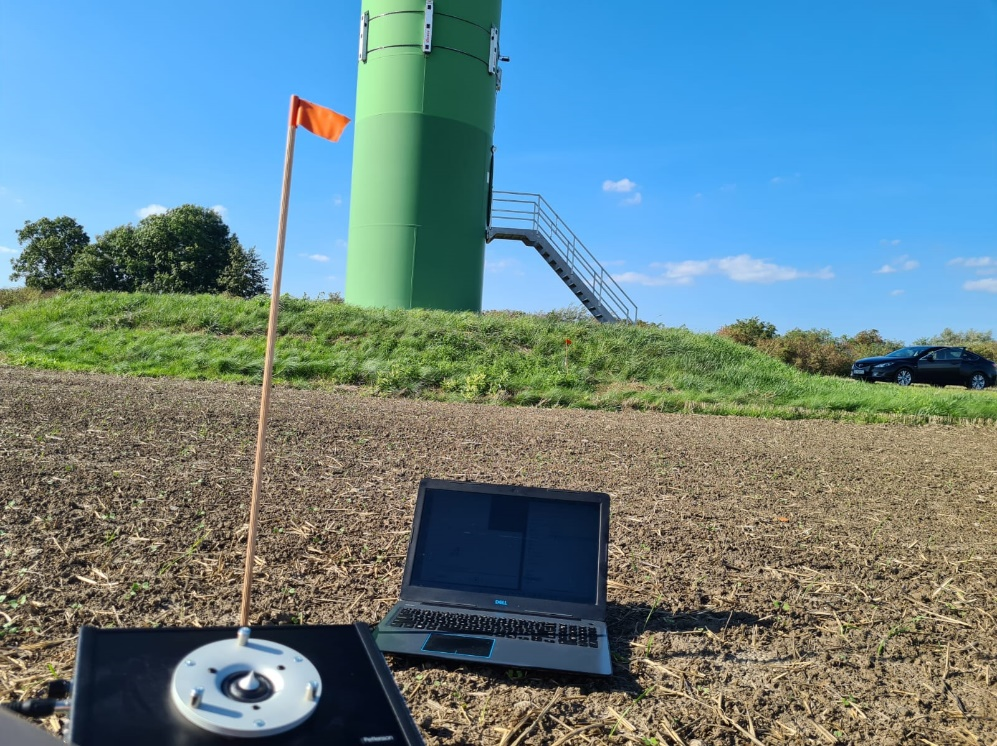
\includegraphics[width=0.8\textwidth]{sprz/fieldtests.png}
  \caption{Testy terenowe systemu SMART z użyciem głośnika Pettersson L400 i laptopa. Źródło: Bioseco}
  \label{img:fieldtests}
\end{figure}

\section{Wyniki testów}
Każda częstotliwość w każdej odległości i pod każdym kątem od mikrofonu została wyemitowana trzykrotnie (w większości przypadków). W wynikach uwzględniono jaki procent głosów w danej lokalizaci został wykryty, np. jeśli wykryto 2 odtworzenia na 4, to oznaczano wykrycie 50\% dźwięków.

Poniższe wykresy ilustrują odległości detekcji dźwięku w poszczególnych konfiguracjach odległości i kąta, w podziale na poszczególne częstotliwości (\ref{img:angle0}, \ref{img:angle30}, \ref{img:angle60}, \ref{img:angle90}).

  \begin{figure}[h]
    \centering
    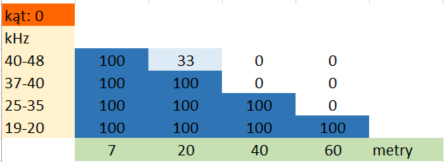
\includegraphics[width=0.8\textwidth]{sprz/angle0.png}
    \caption{Odległości detekcji dla poszczególnych częstotliwości pod kątem 0\textdegree do przodu mikrofonu.}
    \label{img:angle0}
  \end{figure}
\clearpage

  \begin{figure}[h]
    \centering
    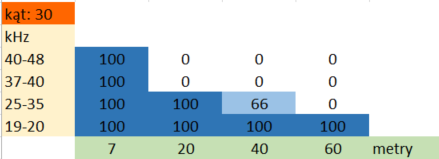
\includegraphics[width=0.8\textwidth]{sprz/angle30.png}
    \caption{Odległości detekcji dla poszczególnych częstotliwości pod kątem 30\textdegree do przodu mikrofonu.}
    \label{img:angle30}
  \end{figure} 

  \begin{figure}[h]
    \centering
    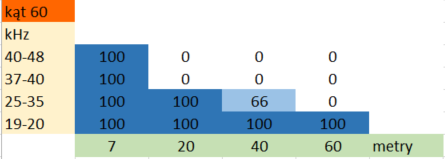
\includegraphics[width=0.8\textwidth]{sprz/angle60.png}
    \caption{Odległości detekcji dla poszczególnych częstotliwości pod kątem 60 do przodu mikrofonu.}
    \label{img:angle60}
  \end{figure} 

  \begin{figure}[h]
    \centering
    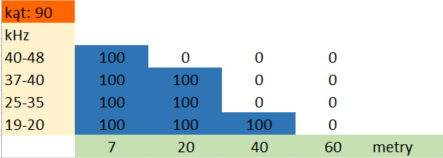
\includegraphics[width=0.8\textwidth]{sprz/angle90.png}
    \caption{Odległości detekcji dla poszczególnych częstotliwości pod kątem 90\textdegree do przodu mikrofonu.}
    \label{img:angle90}
  \end{figure}

\newpage
Na podstawie tych wyników można zauważyć następujące prawidłowości:
\begin{itemize}
  \item{Odległość detekcji ultradźwięków jest największa dla najniższych częstotliwości i maleje wraz ze wzrostem częstotliwości. Maksymalna odległość dotyczy częstotliwości 16-20 kHz i wynosi do 60 m, a najmniejsza odległość dla częstotliwości 37-48 kHz i wynosi do 20 m. Oznacza to, że gatunki takie jak borowiec i borowiaczek są wykrywane z odległości do 60 m, a karliki i inne nietoperze o wysokiej częstotliwości z maksymalnie 20 m.,}
  \item{Gdyby progi odległości były mniejsze, odległości wykrywania byłyby dokładniejsze i w większości przypadków wyższe,}
  \item{Częstotliwości 16-35 kHz są wykrywane równie dobrze, gdy dźwięki emitowane są pod kątem od 0\textdegree do 60\textdegree, wykrywalność zmniejsza się o 20-33\%, gdy dźwięki są emitowane pod kątem 90\textdegree,}
  \item{Dla wyższych częstotliwości – 37-48 kHz, większe znaczenie może mieć kąt padania dźwięku, gdyż w przypadku kątów 30\textdegree i 60\textdegree odległość detekcji zmniejsza się o ponad 50\% w porównaniu do kąta 0\textdegree. Niemniej jednak w przypadku częstotliwości 37-40 kHz przy 90\textdegree wykrywalność jest taka sama jak przy kącie 0\textdegree, dlatego wnioski nie są do końca jednoznaczne. Nie badano także odległości 10 i 15 m, co w tym przypadku mogłoby znacząco poprawić uzyskiwane pokrycie odległości.}
\end{itemize}

Maksymalne odległości detekcji nietoperzy odzywających się w poszczególnych zakresach częstotliwości odpowiadają odległościom obliczonym matematycznie dla tych częstotliwości \cite{agranat}, co pozwala ocenić, że system SMART wykrywa nietoperze z dużą skutecznością.

\section{Propozycja liczby i rozmieszczenia mikrofonów}
W celu przygotowania planu liczby i rozmieszczenia mikrofonów na turbinie wiatrowej wykorzystano informacje z konslutacji z firmą Wildife Acoustics oraz testów ternowych przeprowadzonych w ramach niniejszej pracy.

Z uwagi na dobre pokrycie kąta 180\textdegree przez jeden mikrofon, użycie dwóch mikrofonów na jednej wysokości pokryje kąt 360\textdegree.

Z uwagi na krótkie zasięgi wykrywania nietoperzy mikrofony powiny być zlokalizowane jak najbliżej łopat turbiny, tak by wykrywać aktywność w miejscu, w którym ich obecność może wiązać się z kolizjami, czyli w gondoli lub w dolnym zakresie łopaty. Z punktu widzenia ochrony nietoperzy optymalnym byłby montaż jednego lub dwóch mikrofonów w gondoli, i jednego lub dwóch w dolnym zasięgu łopaty na wieży. Ze względów praktycznych montaż oraz poźniejszy dostęp do mikrofonów na poziomie dolnego zasięgu łopaty będzie drogi z uwagi na konieczny dostęp linowy oraz kłopotliwy z uwagi na brak opracowanego sposobu montażu w tym miejscu. Dlatego na obecnym etapie montaż powinien mieć miejsce w gondoli, bądź poprzez wywiercenie otworu w gondoli bądź montaż na szczycie gondoli na elementach takich jak barierki itp.
Mikrofon, bądź mikrofony wraz z kontrolerem powinny znajdować się razem w gondoli, gdyż długość kabla Ethernet jakiego można użyć do połączenia mikrofonu z kontrolerem wynosi 100 m, z uwagi na poprawność przesyłu danych. Gdy odległość od gondoli do podstawy wiatraka jest mniejsza niż 100 m, kontroler może znajdować się na dole wieży.

Odległości detekcji nietoperzy są na tyle małe w kontekście ich ochrony przed kolizjami z turbinami wiatrowymi, że klasyczne podejście oparte o system detekcyjno-reakcyjny polegające na wyłączeniu turbiny na podstawie każdego pojedynczego przelotu nie będzie przydatne, lecz konieczne będzie dobranie specyficznego wyzwalacza zatrzymującego i ponownie uruchamiającego turbinę, którym może być np. liczba zarejestrowanych przelotów nietoperzy w określonej jednostce czasu. W wyzwalaczach zatrzymań można użyć dodatkowo warunków środowiskowych, takich jak prędkość wiatru czy występowanie opadów (po połączeniu systemu SMART z systemem SCADA turbiny wiatrowej). Minimalizacje z zastosowaniem ograniczenia pracy turbin w określonych warunkach wiatrowych i opadów są obecnie stosowane w celu ograniczenia śmiertelności na farmach wiatrowych \cite{Wytyczne}


\chapter{Struktura systemu}

Struktura wytworzonego systemu została przedstawiona w podziale na poszczególne komponenty.

\section{Schemat połączeń}
System SMART na turbinie wiatrowej połączony jest do sieci internetowej, gdzie skonfigurowane jest połączenie do sieci Bioseco. Komputer firmowy, na którym skonfigurowane jest połączenie do sieci Bioseco przez VPN łączy się zdalnie z systemem SMART, dzięki czemu możliwy jest dostęp do danych z mikrofonu (\ref{img:system-connection}).

\begin{figure}[h] 
  \centering
  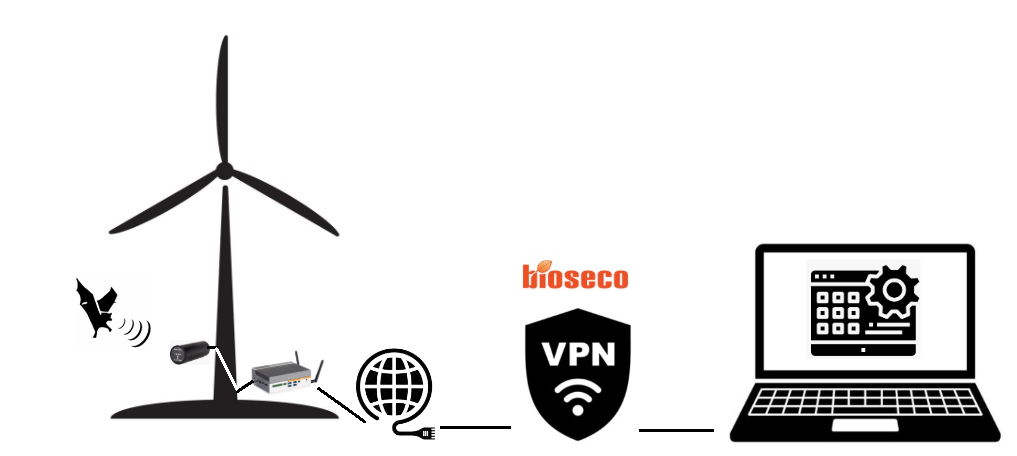
\includegraphics[width=0.8\textwidth]{sprz/system-connection.png}
  \caption{Schemat połączeń sieciowych pomiędzy systemem SMART i komputerem, na którym uruchomiona jest aplikacja.}
  \label{img:system-connection}
\end{figure} 


\section{Architektura systemu}

Na poniższych modelach przedstawiono najważniejsze elementy logiczne, urządzenia wejścia-wyjścia oraz obieg informacji w systemie (\ref{img:architektura_systemu2}). W celu ułatwienia zrozumienia osadzenia systemu w rzeczywistości, architekturę zobrazowano również w postaci graficznej, łącznie z widokiem interfejsu (\ref{img:reprezentacja_graficzna}). 

\begin{figure}[h]
    \centering
    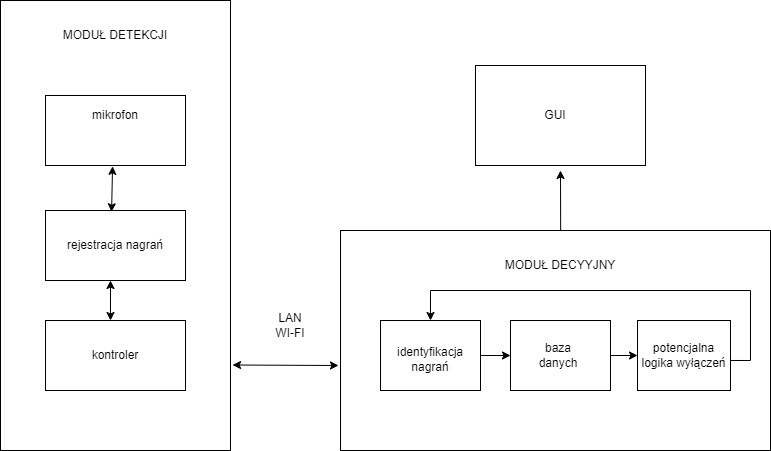
\includegraphics[width=1.0\textwidth]{sprz/architektura_systemu2.png}
    \caption{Logiczny model architektury systemu}
    \label{img:architektura_systemu2}
\end{figure}
\clearpage

\begin{figure}[h]
    \centering
    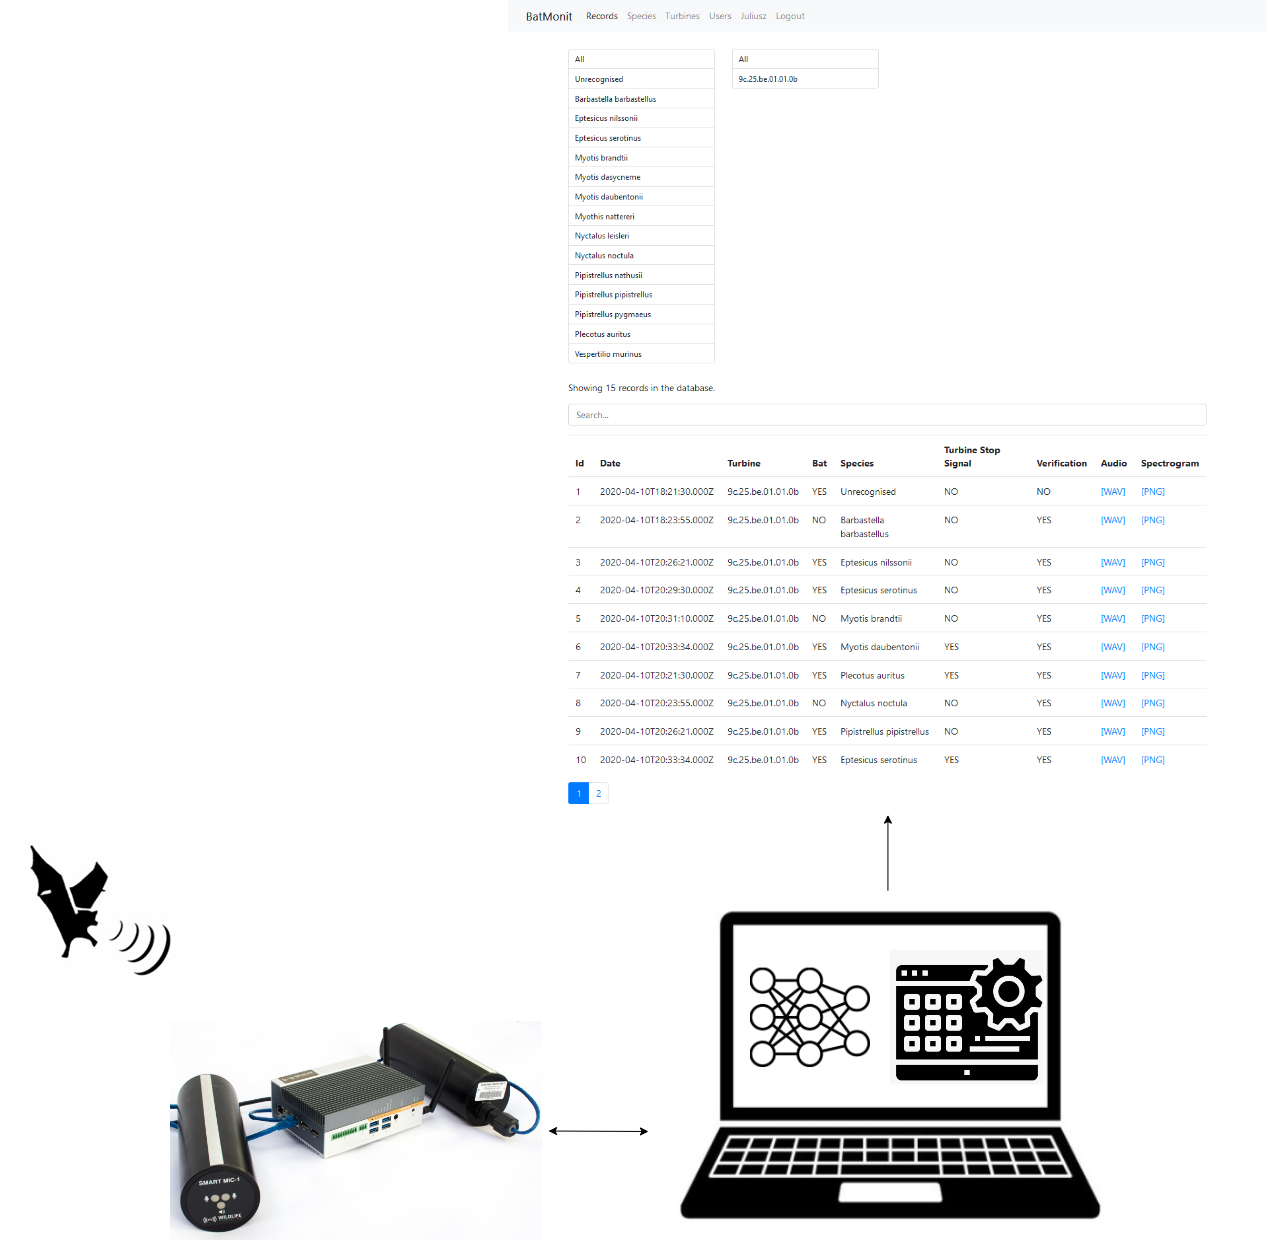
\includegraphics[width=1.0\textwidth]{sprz/graficzna-reprezentacja-systemu.png}
    \caption{Graficzna reprezentacja architektury systemu}
    \label{img:reprezentacja_graficzna}
\end{figure}

\section{Hardware}
Kluczowe zasoby sprzętowe rozwiązania, to system SMART firmy Wildlife Acoustics. Składa się on z mikrofonu ultradźwięków oraz tzw. kontrolera, będącego prostym przemysłowym komputerem. Mikrofon jest połączony z kontrolerem kablem Ethernet, co pozwala na zasilanie mikrofonu oraz przesył danych pomiędzy tymi komponentami. Dane z mikrofonu pobierane są przez oprogramowanie Wildlife Acoustics zainstalowane na kotrolerze i tam też są one gromadzone.
\clearpage

\begin{figure}[h]
  \centering
  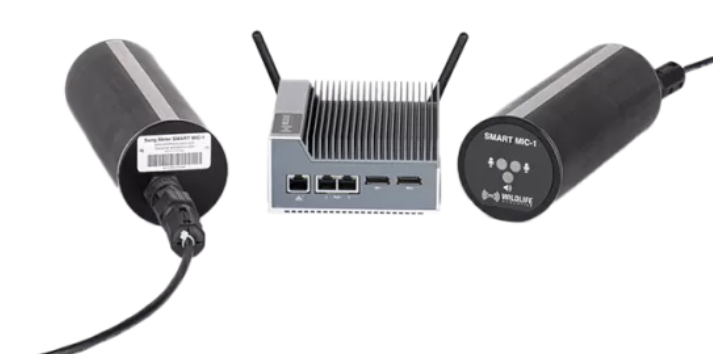
\includegraphics[width=0.8\textwidth]{sprz/smart2}
  \caption{system SMART - mikrofon ultradźwięków i kontroler}
  \label{img:smart2}
\end{figure}

\section{Model sieci neuronowej}
Do treningu i predykcji gatunków nietoperzy użyta został sieć konwolucyjna składająca się z czterech bloków konwolucyjnych (z warstwą konwolucyjną, funkcją aktywacji ReLU i warstwą max-pooling), warstwy spłaszczającej do przestrzeni jednowymiarowej (warstwa flatten), warstwy fully-connected (w PyTorch nazywaną "linear") oraz ostatniej warstwy softmax, pozwalającej na uzyskanie wartości prawdopodobieństw przynależności nagrania do danej klasy (gatunku nieoperza).

W każdej z warstw konwolucyjnych zastosowano funkcję aktywacji ReLU i warstwę max-pooling o filtrze w rozmiarze 2 ("stride").
\clearpage

\section{Aplikacja użytkownika}

Aplikacja użytkownika służy użytkownikowi do przeglądania rekordów tworzonych przez model na podstawie zarejestrowanych nagrań. Do celu nawigacji po aplikacji służy pasek menu w górnej części ekranu, który zawiera odnośniki do poszczególnych widoków.

Widok rejestracji (\ref{img:app_register}) pozwala na zarejestrowanie nowego użytkownika. Po dokonaniu rejestracji nowy użytkownik automatycznie zostaje zalogowany. Po zalogowaniu w pasku menu pojawia się przycisk \textit{Logout} służący do wylogowania aktualnie zalogowanego użytkownika.
\begin{figure}[h]
  \centering
  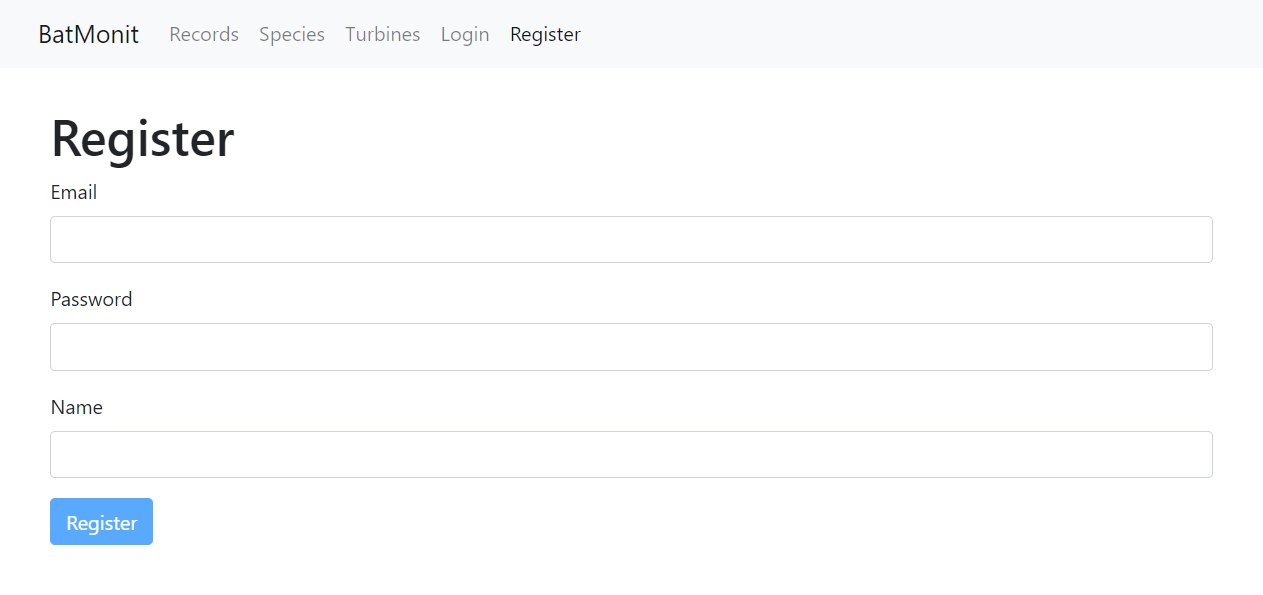
\includegraphics[width=0.8\textwidth]{sprz/app_register}
  \caption{Widok rejestracji użytkownika}
  \label{img:app_register}
\end{figure}
\clearpage

Do celu zalogowania istniejącego już użytkownika służy widok logowania (\ref{img:app_login}).
\begin{figure}[h]
  \centering
  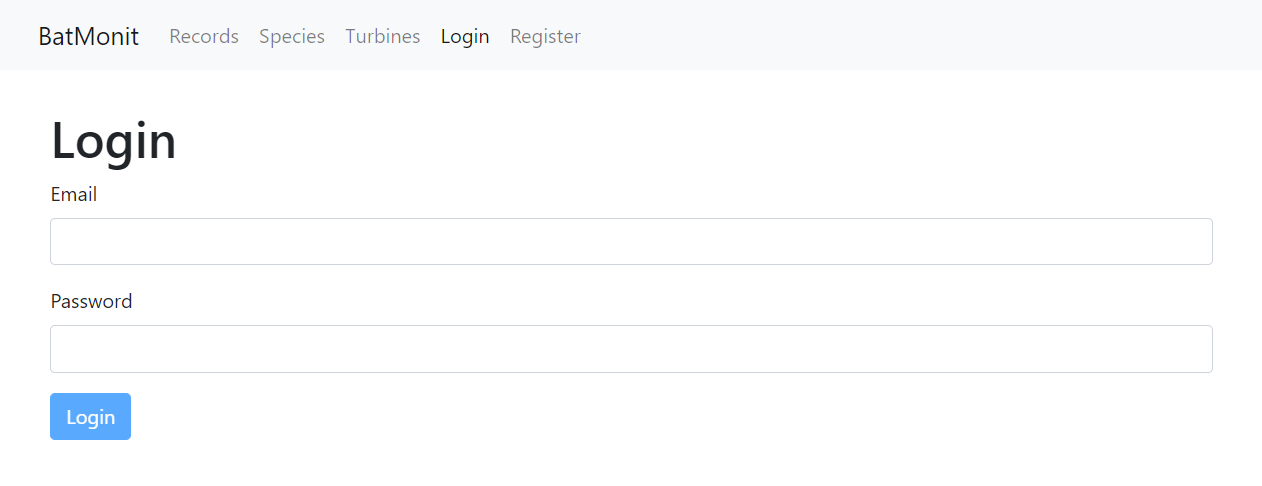
\includegraphics[width=0.8\textwidth]{sprz/app_login}
  \caption{Widok logowania użytkownika}
  \label{img:app_login}
\end{figure}
\clearpage

Linki \textit{Login} i \textit{Register} są widoczne w pasku menu tylko w razie, gdy żaden użytkownik nie jest zalogowany.

Użytkownicy dzielą się na użytkowników zwykłych oraz na użytkowników z prawami administracyjnymi. W razie zalogowania użytkownika o zwykłych prawach obok przycisku \textit{Logout} pojawia się przycisk z podaną przy logowaniu nazwą użytkownika (\ref{img:app_menu_regular_user}).

\begin{figure}[h]
  \centering
  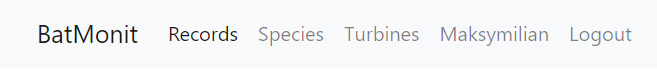
\includegraphics[width=0.8\textwidth]{sprz/app_menu_regular_user}
  \caption{Widok menu dla zwykłego użytkownika}
  \label{img:app_menu_regular_user}
\end{figure}
\clearpage

W przypadku zalogowania użytkownika z prawami administracyjnymi w pasku menu widoczny jest również przycisk \textit{Users} do widoku listy wszystkich istniejących użytkowników (\ref{img:app_users}.

\begin{figure}[h]
  \centering
  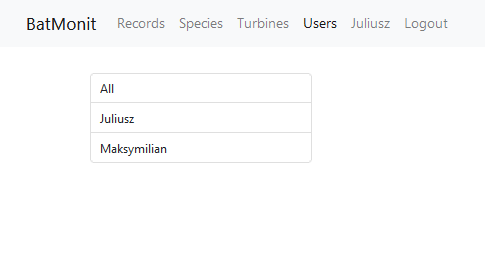
\includegraphics[width=0.8\textwidth]{sprz/app_users}
  \caption{Widok listy użytkowników}
  \label{img:app_users}
\end{figure}
\clearpage

Widok rekordów (\ref{img:app_records} dzieli się na komponenty odpowiedzialne za filtrowanie wyników w górnej części oraz tabelę wyników w dolnej części.

W górnej części widoku rekordów znajduje się panel filtrów z listą wszystkich gatunków nietoperzy. Kliknięcie na któryś z wymienionych gatunków filtruje listę rekordów i wyświetla tylko rekordy zawierające wybrany gatunek. Domyślny wybór fitrowania to \textit{All}, czyli wyświetlanie wszystkich rekordów.

Poniżej panelu filtrów znajduje się komunikat podsumowujący liczbę istniejących w bazie danych rekordów według aktualnie wybranych kryteriów. W razie braku rekordów do wyświetlenia, w tym miejscu znajduje się komunikat o tej treści.

Pod komunikatem znajduje się okno wyszukiwania, które przyjmuje dane wejściowe od użytkownika i pozwala na wyszukiwanie po zawartości tabeli \textit{Date}.

W nagłówku tabeli zawierającej listę rekordów według aktualnych kryteriów filtrowania znajdują się nazwy poszczególnych kolumn odpowiadających nazwom kolumn w bazie danych. Kliknięcie na nazwię kolumny sortuje wyniki po zawartości tej kolumny w kolejności rosnącej lub malejącej, zaś ponowne kliknięcie odwraca kolejność na przeciwną.

Pod tabelą rekordów znajdują się przyciski paginacji, które pozwalając podzielić listę rekordów na osobne strony i wyświetlić zawartość kolejnych stron. Ilość przycisków stron generowana jest dynamicznie w zależności od ilości rekordów spełniających wybrane kryteria wyszukiwania oraz ilości rekordów wyświetlanych na jednej stronie.

\begin{figure}[h]
  \centering
  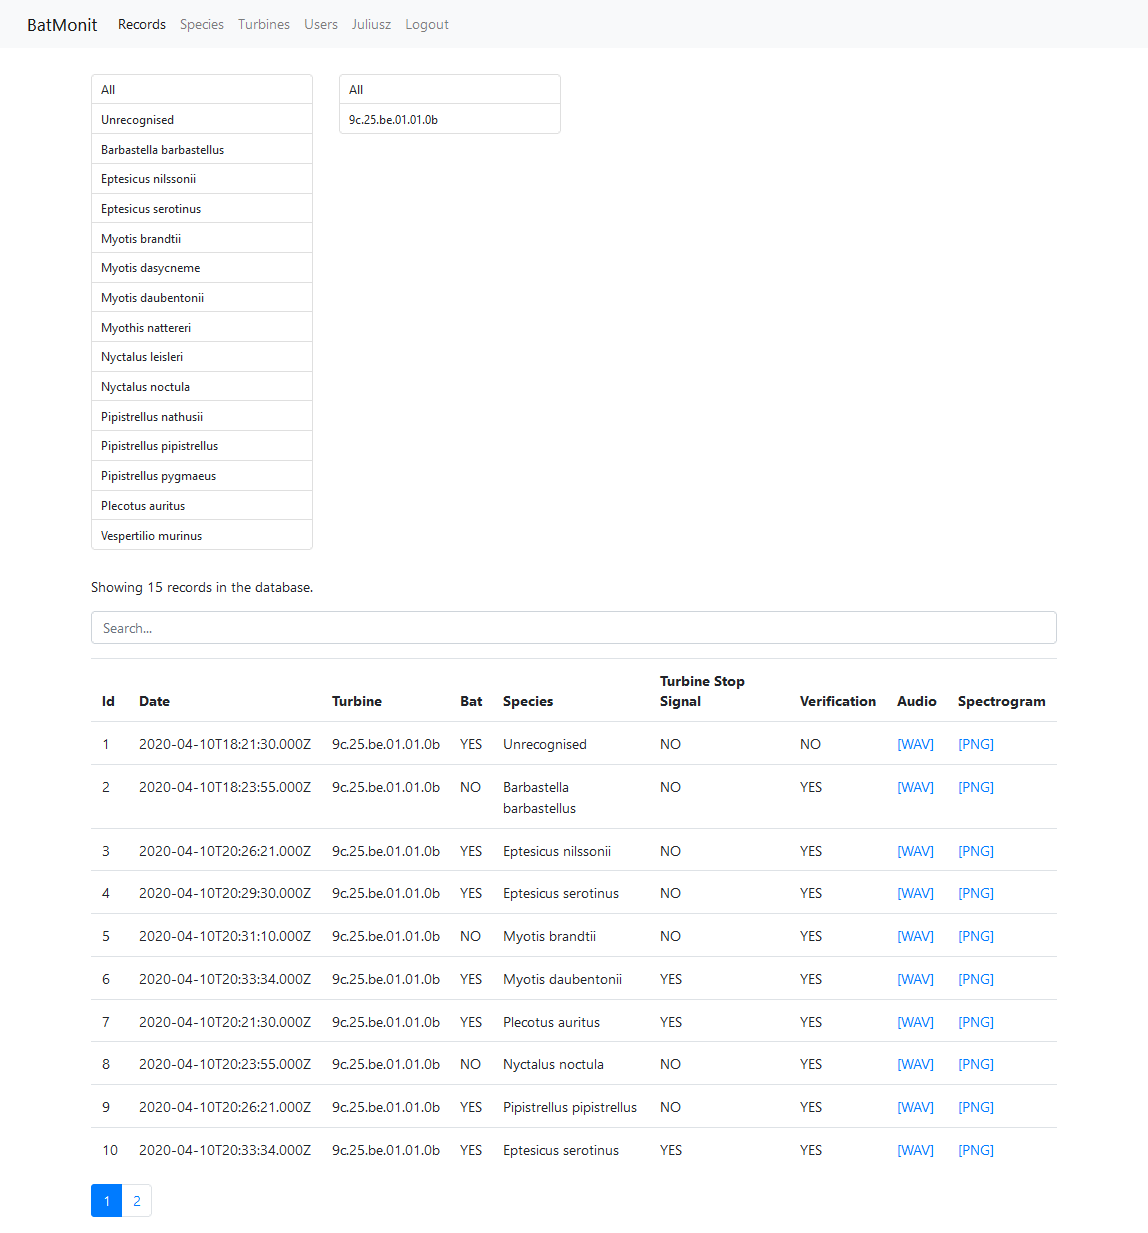
\includegraphics[width=0.8\textwidth]{sprz/app_records}
  \caption{Widok listy rekordów}
  \label{img:app_records}
\end{figure}

\chapter{Realizacja sieci neuronowej}

\section{Przygotowanie danych}
Przygotowanie danych obejmowało podpisanie nagrań zgodnie z wykazem gatunków nietoperzy przypisanych do danych nagrań, które znajdowały się w pliku CSV.

\subsection{Dobór typu spektogramu}
Do treningu użyto dźwięków przetworzonych na obrazy. Rozważano użycie zwykłego spektrogramu i mel-spectrogramu, jednak zdecydowano się na użycie zwykłego spectrogramu, ponieważ dawał on lepszy obraz. W przypadku bardzo delikatnych głosów nietoperzy na mel-spectrogramie pulsy były często niewidoczne.

\subsection{Cięcie}
W celu uzyskania jednolitych wielkości danych na wejściu wszystkie nagrania pociąto na odcinki dwusekundowe. W przypadku gdy ostatni element był krótszy niż dwie sekundy uzupełniano tę część zerami.

\section{Dobór sieci neuronowej}
Po przeglądzie literatury, konsultacjach z ekspertami oraz weryfikacji zasobów czasowych zdecydowano się ostatecznie na użycie konwolucyjnej sieci neuronowej jako sieci przystępnej w implementacji a jdnocześnie potencjalnie dającej dobre wyniki.

\subsection{Przegląd literatury}


\section{Dobór parametrów sieci neuronowej}

\subsection{Parametry warstw sieci}
Sieć konwolucyjna składa się z czterech bloków konwolucyjnych (z warstwą konwolucyjną, funkcją aktywacji ReLU i warstwą max-pooling), warstwy spłaszczającej do przestrzeni jednowymiarowej (warstwa "flatten"), warstwy fully-connected (w PyTorch nazywaną "linear") oraz ostatniej warstwy softmax, pozwalającej na uzyskanie wartości prawdopodobieństw przynależności nagrania do danej klasy (gatunku nieoperza).

Parametry pierwszej warstwy konwolucyjnej:
\begin{itemize}
  \item{liczba kanałów na wejściu - 1}
  \item{liczba kanałów na wyjściu (i liczba filtrów) - 16,}
  \item{rozmiar filtra ("kernel size") - 3,}
  \item {przsunięcie filtra ("stride") - 1,}
  \item{uzupełnienie skrajnych wartości ("padding") - 2.}
\end{itemize}


Parametry drugiej warstwy konwolucyjnej:
Warstwa konwolucyjna
\begin{itemize}
  \item{liczba kanałów na wejściu - 16}
  \item{liczba kanałów na wyjściu (i liczba filtrów) - 32,}
  \item{rozmiar filtra ("kernel size") - 3,}
  \item {przsunięcie filtra ("stride") - 1,}
  \item{uzupełnienie skrajnych wartości ("padding") - 2.}
\end{itemize}


Parametry trzeciej warstwy konwolucyjnej:
\begin{itemize}
  \item{liczba kanałów na wejściu - 32}
  \item{liczba kanałów na wyjściu (i liczba filtrów) - 64,}
  \item{rozmiar filtra ("kernel size") - 3,}
  \item {przsunięcie filtra ("stride") - 1,}
  \item{uzupełnienie skrajnych wartości ("padding") - 2.}
\end{itemize}

Parametry czwartej warstwy konwolucyjnej:
\begin{itemize}
  \item{liczba kanałów na wejściu - 64}
  \item{liczba kanałów na wyjściu (i liczba filtrów) - 128,}
  \item{rozmiar filtra ("kernel size") - 3,}
  \item {przsunięcie filtra ("stride") - 1,}
  \item{uzupełnienie skrajnych wartości ("padding") - 2.}
\end{itemize}


W każdej z warstw konwolucyjnych zastosowano funkcję aktywacji ReLU i warstwę max-pooling o filtrze w rozmiarze 2 ("stride").

\subsection{Funkcje aktywacji}
Funkcja aktywacji używana jest do obliczania wartości neuronów w warstwach wyjściowych.

W warstwach konwolucyjnych jako funkcji aktywacji użyto funkcji ReLU. (Rectified Linear Unit). Jest to najczęściej używana faunkcja aktywacji w warstwach ukrytych. Do jej zalet należą szybkość i nieliniowość.

W ostatniej warstwie użyto funkcji aktywacji softmax. Przekształca ona wartości uzyskiwane na wyjściu tak, aby ich suma była równa 1, dzięki czemu dobrze modeluje prawdopodobieństwo. Jest to najczęsciej wykorzystywana funkcja w warstwach wyjściowych.

\subsection{Funkcja błędu}
Funkcja ta jest często używana w sieciach neuronowych w problemach klasyfikacji. Określa ona jak dobrze model przewiduje klasy - im mniejsza wartość funkcji błędu, tym większa dokładnosć modelu. Podczas uczenia się sieci dąży się do zmniejszania wartości fukcji błędu. W sieci neuronowej użytej w niniejszej pracy wykorzystano funkcję entropii krzyżowej.

\subsection{Optymalizator}
Optymalizator jest to funkcja lub algorytm decydująca o tym jak zmienić wagi sieci na podstawie funkcji błędu, tak aby zmniejszyć wartość tej funkcji. Optymalizator wływa na to jak szybko sieć będzie się uczyć poprzez zmianę jej parametrów oraz jak poradzi sobie z problemami takimi jak utknięcie w lokalnym minimum. W sieci neuronowej przedstawionej w niniejszej pracy wykorzystano optymalizator Adam (Adaptive Moment Estimation). Optymalizotor ten jest najczęsciej wykorzystywanym i dającym najczęściej najlepsze wyniki.

\section{Architektura sieci neuronowej i modułów związanych z teningiem sieci}
Sieć neuronowa napisana została w języku Python, z użyciem bilbiotek PyTorch oraz TorchAudio. 


PyTorch jest biblioteką oferującą narzędzia do budowy i trenowania sieci neuronowych, zawiera m.in. moduły do tworzenia warstw sieci, funkcji stratu czy optymalizatorów, daje wsparcie do trenowania na kartach graficznych \cite{pytorch}.
PyTorch jest biblioteką o podobnej popularności co Tensorflow, a w ostatnich latach nawet częściej wykorzystywaną, szczególnie w środowiskach akademickich. Umożliwia ona na większą elastyczność w budowie sieci i ustawieniach jej parametrów. Do zalet takiego rozwiązania należy większy wpływ na kształt i funkcjonowanie sieci, a do wad - dłuższy czas przygotowania oraz wyższy próg wejścia. 

Biblioteka TorchAudio jest częścią ekosystemu PyTorch i służy do obsługi i obróbki plików dźwiękowych. Dostarcza narzędzi pomocnych w ładowaniu danych audio oraz transformacjach takich jak zmiany prędkości czy głośności, przetwarzanie na spectrogramy czy mel-spectrogramy \cite{torchaudio}. 

Sień neuronowa przygotowana w ramach niniejszej pracy dyplomowej składa się z czterech głównych elementów: modułu transformującego dźwięk do spectrogramów, modułu ładującego dane, modułu do treningu oraz modułu do predykcji.

\subsection{Konwersja dźwięków na spektrogramy}

\begin{lstlisting}[language=Python,caption={Implementacja konwersji dźwięku na spektrogram}, label={lst:audio-to-spectrogram}]
  waveform, sample_rate = torchaudio.load(r'C:\\Users\\Jakub\Documents\\PJATK\\INZ\Batmonit_model\\Chiro_sounds_signed\Audio\\PIPNAT\S4U08639_20210731_234142_PIPNAT.wav')
  fragments = torch.split(waveform, split_size_or_sections=2*sample_rate, dim=1)
  
  specgram = torchaudio.transforms.Spectrogram(
          )(fragments[1])
  
  plt.figure(figsize=(12, 8))
  plt.imshow(specgram[0].log2(), aspect='auto', origin='lower')
  plt.show()
\end{lstlisting}


\subsection{Ładowanie danych}

Moduł ładujący dane jest najbardziej rozbudowanym elementem architektury związanej z treningiem sieci. Składa się z wielu funkcji, które zapewniają identyczność parametrów każdego z nagrań, takich jak liczba kanałów czy wielkość obrazu, ....

Główna funkcja tego modułu uruchamia ładowanie danych z uwzględnieniem wszystkich tych elementów.

\begin{lstlisting}[language=Python,caption={Implementacja modułu do ładowania danych}, label={lst:audio-to-spectrogram}]
  if __name__ == "__main__":
  ANNOTATIONS_FILE = r"C:\Users\Jakub\Documents\PJATK\INZ\Batmonit_model\Chiro_sounds_signed\Metadata\Annotations.csv"
  AUDIO_DIR = r"C:\Users\Jakub\Documents\PJATK\INZ\Batmonit_model\Chiro_sounds_signed\Audio"
  SPECTROGRAM_DIR = r"C:\Users\Jakub\Documents\PJATK\INZ\Batmonit_model\Chiro_sounds_signed\Spectrogram"
  SAMPLE_RATE = 192000
  NUM_SAMPLES = 2000000

  if torch.cuda.is_available():
      device = "cuda"
  else:
      device = "cpu"
  print(f"Using device: {device}")

  spectrogram = torchaudio.transforms.Spectrogram(
      n_fft=1024,
      hop_length=1024,
  )
  bd = BatsDataset(ANNOTATIONS_FILE,
                          AUDIO_DIR,
                          SPECTROGRAM_DIR, 
                          spectrogram, 
                          SAMPLE_RATE,
                          NUM_SAMPLES,
                          device)

  print(f"There are {len(bd)} samples in the dataset.")
  signal, label = bd[0]
  print(signal, label)
\end{lstlisting}

\subsection{Sień neuronowa}

\begin{lstlisting}[language=Python,caption={Implementacja sieci neuronowej}, label={lst:Sequelize_validate}]
  class CNNNetwork(nn.Module):

  def __init__(self):
      super().__init__()
      self.conv1 = nn.Sequential(
          nn.Conv2d(
              in_channels=1, 
              out_channels=16,  
              kernel_size=3,  
              stride=1,
              padding=2
          ),
          nn.ReLU(),
          nn.MaxPool2d(kernel_size=2)  
      )
      self.conv2 = nn.Sequential(
          nn.Conv2d(
              in_channels=16,
              out_channels=32,
              kernel_size=3,
              stride=1,
              padding=2
          ),
          nn.ReLU(),
          nn.MaxPool2d(kernel_size=2)
      )
      self.conv3 = nn.Sequential(
          nn.Conv2d(
              in_channels=32,
              out_channels=64,
              kernel_size=3,
              stride=1,
              padding=2
          ),
          nn.ReLU(),
          nn.MaxPool2d(kernel_size=2)
      )
      self.conv4 = nn.Sequential(
          nn.Conv2d(
              in_channels=64,
              out_channels=128,
              kernel_size=3,
              stride=1,
              padding=2
          ),
          nn.ReLU(),
          nn.MaxPool2d(kernel_size=2)
      )
      self.flatten = nn.Flatten()
      self.linear = nn.Linear(128*33*13, 14) 
                                             
      self.softmax = nn.Softmax(dim=1)

  def forward(self, input_data):
      x = self.conv1(input_data)
      x = self.conv2(x)
      x = self.conv3(x)
      x = self.conv4(x)
      x = self.flatten(x)
      logits = self.linear(x)
      predictions = self.softmax(logits)
      return predictions

if __name__ == "__main__":
  cnn = CNNNetwork()
\end{lstlisting}

\subsection{Trenowanie na zbiorze treningowym}

\begin{lstlisting}[language=Python,caption={Implementacja modułu do trenowania sieci}, label={lst:train}]
  if __name__ == "__main__":

  if torch.cuda.is_available():
      device = "cuda"
  else:
      device = "cpu"
  print(f"Using device: {device}")

  spectrogram = torchaudio.transforms.Spectrogram(
      n_fft=1024,
      hop_length=1024,
  )

  bd = BatsDataset(ANNOTATIONS_FILE,
                          AUDIO_DIR,
                          SPECTROGRAM_DIR, 
                          spectrogram, 
                          SAMPLE_RATE,
                          NUM_SAMPLES,
                          device)


  train_data_loader = create_data_loader(bd, batch_size=BATCH_SIZE)

  cnn = CNNNetwork().to(device)

  loss_fn = nn.CrossEntropyLoss()
  optimiser = torch.optim.Adam(cnn.parameters(), lr=LEARNING_RATE)

  train(cnn, train_data_loader, loss_fn, optimiser, device, EPOCHS)

  torch.save(cnn.state_dict(), MODEL_PATH)

  print("Model trained and stored at feedforwardnet.pth")
\end{lstlisting}

\subsection{Przewidywanie wyniku na zbiorze testowym}

\begin{lstlisting}[language=Python,caption={Implementacja modułu do trenowania sieci}, label={lst:train}]
  if __name__ == "__main__":

  cnn = CNNNetwork()
  state_dict = torch.load(r"C:\Users\Jakub\Documents\PJATK\INZ\Batmonit_model\feedforwardnet.pth", map_location=torch.device('cpu'))
  cnn.load_state_dict(state_dict)

  spectrogram = torchaudio.transforms.Spectrogram(
      n_fft=1024,
      hop_length=1024,
  )

  bd = BatsDataset(ANNOTATIONS_FILE,
                          AUDIO_DIR,
                          SPECTROGRAM_DIR, 
                          spectrogram, 
                          SAMPLE_RATE,
                          NUM_SAMPLES,
                          "cpu")

  input, target = bd[0][0], bd[0][1]
  input.unsqueeze_(0)

  predicted, expected = predict(cnn, input, target,
   class_mapping)

  print(f"Predicted: '{predicted}', expected: '{expected}'")
\end{lstlisting}

\section{Skuteczność sieci neuronowej}

\subsection{Macierz pomyłek}

\subsection{Metryki}

\subsection{Learning rate}

\chapter{Implementacja aplikacji użytkownika}

Aplikacja użytkownika służy do zbierania i zapisywania w bazie danych rekordów tworzonych na podstawie decyzji modelu sieci neuronowej, które następnie pozwala wyświetlić na liście z możliwością filtrowania i sortowania ich. W skład aplikacji wchodzą: baza danych, serwer oraz interfejs użytkownika.

Centralną rolę pełni serwer, który pośredniczy w komunikacji z bazą danych i przyjmuje komunikację ze strony modelu sztucznej inteligencji oraz interfejsu użytkownika. Komunikacja ta realizowana jest poprzez interfejs API (application programming interface).

\section{Baza danych}

Wybrana przez autorów projektu technologia bazy danych to MySQL. Jest to jeden z najbardziej rozpowszechnionych systemów relacyjnych baz danych. Do jego zalet należy szeroka obsługa platform i architektur.

Baza danych zawiera tabele records, turbines, species oraz users. Tabela users gromadzi dane zarejestrowanych użytkowników i nie ma relacji z pozostałymi tabelami (\ref{img:db_diagram}).

\begin{figure}[h]
  \centering
  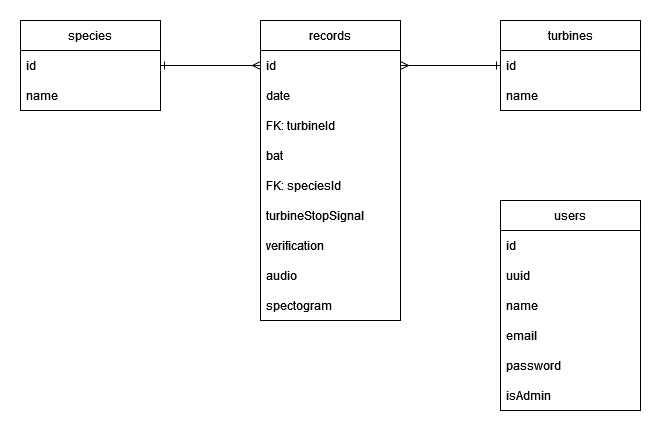
\includegraphics[width=0.8\textwidth]{sprz/db_diagram}
  \caption{Diagram bazy danych}
  \label{img:db_diagram}
\end{figure}
\clearpage

\section{NodeJS}

Serwer aplikacji został napisany w technologii NodeJS \cite{nodejs}. Technologia ta charakteryzuje się relatywnie niskim prógiem wejścia do tworzenia oprogramowania i otwiera programistom pracującym nad frontendem w języku Javascript na wykorzystanie swojej więdzy w tym języku przy pracy w backendzie. Jednocześnie na ujednolicenie pod względem języka oprogramowania części backendowej i frontendowej. Dzięki temu dobrze nadaje się do zastosowania w niniejszym projekcie.

NodeJS to wieloplatformowe środowisko składające się z V8 (silnika Javascript firmy Google), pętli zdarzeń obsługiwanej przez bibliotekę libUV oraz interfejsu do obsługi niskpoziomowego wejścia-wyjścia.

Do zalet NodeJS należy:
\begin{enumerate}
  \item \textbf{Asynchroniczność.} Poprzez nieblokującą obsługę wejścia-wyjścia służy do tworzenia wysoce skalowalnych rozwiązań serwerowych przy maksymalizacji wykorzystania procesora i pamięci.
  \item \textbf{Wysoka skalowalność.} Pętla zdarzeń pozwala uniknąć tworzenia wielowątkowych rozwiązań. Procesy mogą być uruchamiane współbieżnie lub równolegle. Wywołanie zwrotne (ang. callback) sygnalizuje następnie powodzenie lub niepowodzenie zadania.
  \item \textbf{Duża popularność.} Dostępne są tysiące bibliotek o otwartym kodzie źródłowym tworzonych przez środowisko NodeJS.
\end{enumerate}

\section{Biblioteki}

W projekcie użyto następujących otwartych bibliotek, które dostarczyły szeregu funkcjonalności i skróciły czas jego tworzenia:
\begin{itemize}
  \item Sequelize
  \item Express
  \item Jest
  \item Supertest
  \item Joi
  \item Jsonwebtoken
\end{itemize}

\subsection{Sequelize}

Do komunikacji z bazą danych wykorzystano bibliotekę Sequelize \cite{sequelize}. Sequelize to narzędzie mapowania obiektowo-relacyjnego (ang. ORM - Object-Relational Mapping), które pełni rolę "pomostu" pomiędzy aplikacją obiektową a relacyjną bazą danych.
Do zalet ORM należą:
\begin{itemize}
  \item odwzorowanie tabel relacyjnej bazy danych na obiekty w obiektowym języku programowania wykorzystanym w aplikacji
  \item wykonywanie operacji na danych w bazie danych jak na obiektach języka programowania
  \item uniknięcie nadmiarowego kodu
  \item wykorzystanie tego samego kodu aplikacji w komunikacji z różnymi bazami danych
  \item tworzenie zapytań dla wielu tabel
  \item przyspieszenie i uproszczenie procesu wytworzenia aplikacji
\end{itemize}

Biblioteka ta pozwoliła na wyeliminowanie w kodzie potrzeby formułowania zapytań w języku SQL, które jest trudne w utrzymaniu z punktu widzenia programisty i podatne na błędy w treści zapytań. Serwer posiada zdefiniowany model odpowiadający każdej tabeli w bazie danych. Na podstawie modelu biblioteka Sequelize ma informacje potrzebne do stworzenia zapytania w języku SQL. Listing \ref{lst:Sequelize_Record.create} przedstawia przykład przekazania szeregu zmiennych w celu zapisania ich jako nowy rekord w bazie danych.

\begin{lstlisting}[language=Java,caption={Przykład tworzenia rekordu z pomocą biblioteki Sequelize}, label={lst:Sequelize_Record.create}]
  const record = await Record.create({
    date,
    turbineId,
    bat,
    speciesId,
    turbineStopSignal,
    verification,
    audio,
    spectrogram,
  });
\end{lstlisting}

Biblioteka Sequelize oferuje wbudowaną walidację zapytań po zdefiniowanych w modelu typach danych. Istnieje również możliwość tworzenia niestandardowych komunikatów w razie błędu wykrytego przez walidację, co ukazuje listing \ref{lst:Sequelize_validate}.

\begin{lstlisting}[language=Java,caption={Przykład niestandardowego komunikatu walidacji}, label={lst:Sequelize_validate}]
  Record.init(
    {
      date: {
        type: DataTypes.DATE,
        allowNull: false,
        validate: {
          notNull: { msg: "Record must have a date" },
          notEmpty: { msg: "Date must not be empty" },
        },
      },
    }
  );
\end{lstlisting}

Iteracyjne tworzenie projektu programistycznego z relacyjną bazą danych niesie ze sobą duże ryzyko wprowadzenia zmian do bazy danych, które uszkodziłyby jej strukturę i mogłyby doprowadzić do utraty danych. Takie błędne zmiany są trudne to rozpoznania i usunięcia. Biblioteka Sequelize wychodzi na przeciw potrzebie minimalizacji ryzyka przy zmianach w bazie danych poprzez uwzględnianie ich wewnątrz migracji, podobnie do rozwiązań stosowanych w środowisku korporacyjnym (takich jak Hibernate/Liquibase w projektach w języku Java).

Migracja Sequelize jest to funkcja Javascript zawierająca metodę \textit{up} zawierającą kod zmieniający bazę danych oraz metodę \textit{down} specyfikujący kod odwracający zmiany z metody \textit{up}. Migracja jest zawarta wewnątrz pojedynczego pliku o unikalnej nazwie zawierającej datę utworzenia i opis wprowadzanych zmian. Pliki takie biblioteka Sequelize pozwala tworzyć poleceniem w konsoli. Ideą zastosowania migracji jest stworzenie tym sposobem systemu kontroli wersji dla zmian w bazie danych. Każde zmiany w bazie danych powinny zostać poprzedzone utworzeniem pliku migracji i wypełnieniem obu metod. W razie wystąpienia problemów z bazą danych biblioteka Sequelize pozwala za pomocą konsoli na cofanie się w historii zmian i przywrócenie poprzedniego stanu. Przykład migracji ukazuje listing \ref{lst:Sequelize_migration}.

\begin{lstlisting}[language=Java,caption={Przykład pliku migracji}, label={lst:Sequelize_migration}]
  module.exports = {
    async up(queryInterface, DataTypes) {
      await queryInterface.createTable("records", {
        id: {
          allowNull: false,
          autoIncrement: true,
          primaryKey: true,
          type: DataTypes.INTEGER,
        },
      });
    },
    async down(queryInterface, DataTypes) {
      await queryInterface.dropTable("records");
    },
  };
\end{lstlisting}

O ile zmiany w strukturze tabel bazy danych zarządzane są przez migracje, biblioteka Sequelize daje również możliwość masowego zapełniania bazy danych danymi. Jest to szczególnie przydatne przy procesie implementacji. Pozwala na przyspieszenie i zautomatyzowanie procesu operowania danymi testowymi oraz eliminuje potrzebę bezpośredniego wykonywania zapytań w narzędziu zarządzającym bazą danych (jak np. MySQL Workbench). Do tego celu służą pliki seeder, które w istocie są podobne do migracji, lecz w metodach \textit{up} i \textit{down} należy zawierać kod operujący na danych, nie zaś na strukturze tabel bazy danych. Przykład migracji ukazuje listing \ref{lst:Sequelize_seeder}.

\begin{lstlisting}[language=Java,caption={Przykład pliku seeder}, label={lst:Sequelize_seeder}]
  module.exports = {
    async up(queryInterface, Sequelize) {
      await queryInterface.bulkInsert(
        "turbines",
        [
          {
            name: "9c.25.be.01.01.0b",
            createdAt: "2022-07-27 21:04:11",
            updatedAt: "2022-07-27 21:04:11",
          },
        ],
        {}
      );
    },
  
    async down(queryInterface, Sequelize) {
      await queryInterface.bulkDelete("turbines", null, {});
    },
  };
\end{lstlisting}

\subsection{Express}

Serwer w NodeJS do komunikacji z modelem w celu stworzenia rekordów oraz pośredniczenia z interfejsem użytkownika w odczytywaniu zapisanych rekordów wykorzystuje interfejsu API stworzonego z pomocą biblioteki Express \cite{express}.

Biblioteka Express to szablon (ang. framework) dostarczający mechanizmy do:
\begin{itemize}
  \item pisania zapytań HTTP dla różnych ścieżek URL (ang. Uniform Resource Locator)
  \item generowania widoków przez wstawianie danych do modelu
  \item definiowania ogólnych ustawień w aplikacji, jak np. port wykorzystywany do połączenia lub model wykorzystywany do renderowania odpowiedzi
  \item dodawania na dowolnym etapie przetwarzania zapytania wywołania oprogramowania pośredniczącego (ang. middleware)
\end{itemize}

Biblioteka Express pozwoliła na uporządkowanie i czytelne rozmieszczenie zaprogramowanych interfejsów API w imię zasady pojedynczej odpowiedzialności.

\subsection{Joi}

Do walidacji treści wpisywanej przez użytkownika aplikacji przy rejestracji lub logowaniu posłużyła biblioteka Joi. Dostarcza ona wygodny i czytelny szablon tworzenia warunków walidacyjnych. W razie ich niespełnienia przez walidowaną treść któregoś z warunków, zwracany jest błąd o określonej treści. W odróżnieniu od walidacji oferowanej przez bibliotekę Sequelize, Joi pozwala na walidację bardziej wysokopoziomową i nie jest wiązana modelem tworzącym bazę danych.

Listing \ref{lst:Joi} przedstawia wykorzystanie biblioteki Joi wewnątrz funkcji pośredniczącej do potwierdzania toższamości użytkownika.

\begin{lstlisting}[language=Java,caption={Przykład wykorzystania Joi}, label={lst:Joi}]
  function validate(req) {
    const schema = Joi.object({
      email: Joi.string().min(5).max(255).required().email(),
      password: Joi.string().min(5).max(255).required(),
    });
  
    return schema.validate(req);
  }
\end{lstlisting}

\subsection{Jsonwebtoken}

Biblioteka Jsonwebtoken dostarcza metody to generowania i walidowania tzw. tokenów, czyli zaszyfrowanych kluczy. Po udanym logowaniu użytkownika generowany i przesyłany wewnątrz odpowiedzi jest token. Następnie token ten przechowywany jest przez przeglądarkę i dodawany do kolejnych zapytań w komunikacji między interfejsem użytkownika a serwerem poprzez interfejs API. Serwer sprawdza za każdym razem, czy przychodzące zapytanie posiada właściwy token, a w przeciwnym wypadku odmawia przesłania odpowiedzi.

\subsection{Jest}

Za szablon do pisania testów jednostkowych (ang. unit test) posłużyła biblioteka Jest. Jest to popularna biblioteka do testowania rozwiązań w języku Javascript, dostarczająca szablony pisania testów i metody asercji. Dodatkowo biblioteka ta dostarcza narzędzia do analizy i wygenerowania raportu procentowego stopnia pokrycia testami (ang. test coverage) całego kody aplikacji. Pozwala w ten sposób łatwo ustalić, które części aplikacji wymagają jeszcze utworzenia testów. Rysunek (\ref{img:test_coverage}) ukazuje przykładowy raport pokrycia testami.

\begin{figure}[h]
  \centering
  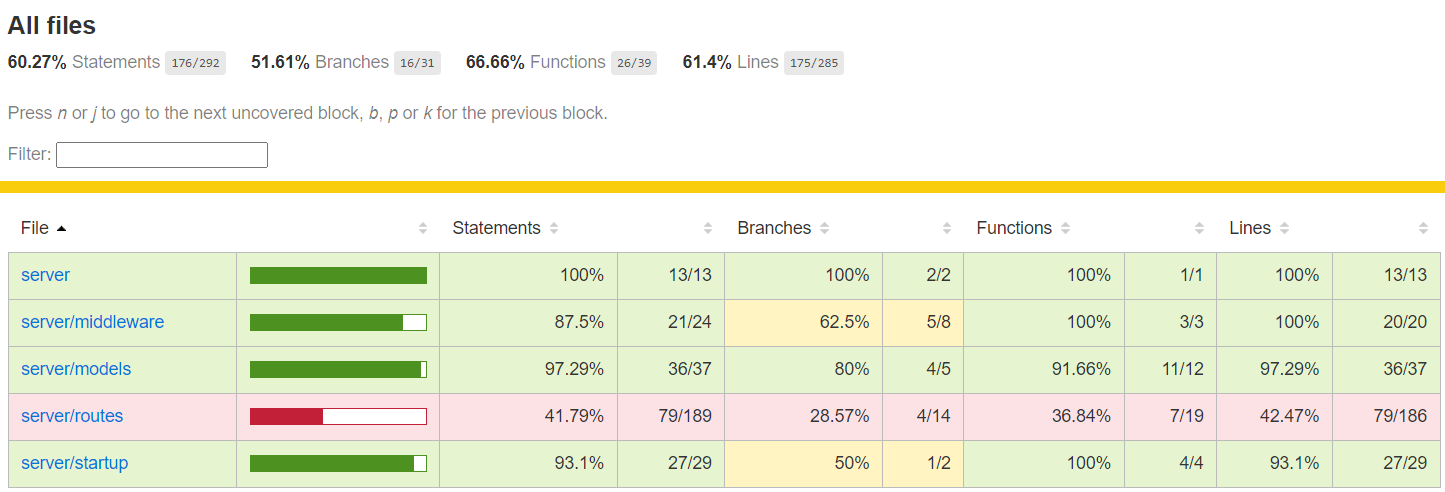
\includegraphics[width=0.8\textwidth]{sprz/test_coverage}
  \caption{Przykładowy raport pokrycia testami}
  \label{img:test_coverage}
\end{figure}

Listing \ref{lst:Jest_unit_test} przedstawia przykład testu jednostkowego z wykorzystaniem biblioteki Jest.

Metoda \textit{describe} pozwala podzielić testy na zestawy odpowiadające konkretnej funcjonalności. Metoda \textit{it} definiuje pojedynczy przypadek testowy, a sama jej nazwa czytana w języku angielskim nakierowuje na zgodne z konwencją nazywanie przypadku testowego w formie słownego opisu spodzewanego wyniku.

\begin{lstlisting}[language=Java,caption={Test jednostkowy z wykorzystaniem Jest}, label={lst:Jest_unit_test}]
  describe("auth middleware", () => {
    it("should populate req.user with the payload of a valid JWT", () => {
      const user = {
        uuid: new DataTypes.UUIDV4(),
        name: "Username",
        isAdmin: true,
      };
      const token = generateAuthToken(user);
      const req = {
        header: jest.fn().mockReturnValue(token),
      };
      const res = {};
      const next = jest.fn();
  
      auth(req, res, next);
  
      expect(req.user).toMatchObject(user);
    });
  });
\end{lstlisting}

\subsection{Supertest}

Biblioteka Supertest w połączeniu z biblioteką Jest posłużyła do utworzenia testów integracyjnych. W projekcie posłużyła ona do testowania działania interfejsów API.

Listing \ref{lst:Supertest} przedstawia przykład testu integracyjego z wykorzystaniem biblioteki Jest. Dostarczana przez bibliotekę Jest metoda \textit{beforeEach} zawiera kod wykonywany przed każdym przypadkiem testowym, zaś metoda \textit{afterEach} po każdym przypadku testowym.

\begin{lstlisting}[language=Java,caption={Test integracyjny z wykorzystaniem Supertest i Jest}, label={lst:Supertest}]
  describe("/api/records", () => {
    beforeEach(async () => {
      server = require("../../index");
    });
    afterEach(async () => {
      await server.close();
      await Record.truncate();
    });
  
    describe("GET /", () => {
      it("should return all records", async () => {
        const res = await request(server).get("/api/records");
  
        expect(res.status).toBe(200);
      });
    });
  });
\end{lstlisting}

\section{ReactJS}

Interfejs użytkownika został napisany w języku Javascript przy wykorzystaniu biblioteki ReactJS, jednej z najbardziej popularnych bibliotek do tworzenia interfejsów graficznych.

Stosowanie biblioteki ReactJS oferuje wiele korzyści:
\begin{enumerate}
  \item \textbf{Tworzenie dynamicznych aplikacji internetowych.} Wymaga napisania mniejszej ilości kodu i oferuje więcej funkcjonalności w odróżnieniu do pracy z samym językiem Javascript.
  \item \textbf{Lepsza wydajność.} Wykorzystując wirtualny DOM (ang. Document Object Model) pozwala na porównywanie poprzedniego stanu każdego komponentu i odświeżanie tylko tych komponentów, które uległy zmianie, w przeciwieństwie do odświeżania wszystkich komponentów. Dzięki temu aplikacje stworzone w ReactJS są bardziej responsywne, szybciej się ładują. Na przykład, ReactJS pozwala na proste korzystanie w tworzonym interfejsie graficznym z asynchroniczności, w której reakcja na akcję użytkownika może być natychmiastowa, a komponent oczekujący na dane nie wstrzymuje aplikacji i wyświetli je, kiedy tylko je otrzyma.
  \item \textbf{Komponenty wielokrotnego użytku.} Aplikacja w ReactJS składa się z wielu komponentów. Każdy z nich posiada logikę, która może zostać wielokrotnie wykorzystana w innym miejscu aplikacji, co pozwala na skrócenie czasu tworzenia aplikacji. Ponadto, podział na komponenty pozwala na funkcjonalne uporządkowanie kodu i poprawienie jego czytelności.
  \item \textbf{Jednokierunkowy przepływ danych.} ReactJS przestrzega jednokierunkowego przepływu danych. Oznacza to, że dane są przekazywane tylko w dół hierarchii od komponentów nadrzędnych do dziedziczących. Widok aplikacji jest rezultatem stanu danych. Stan danych zmienia się pod wpływem akcji. Gdy następują akcje, stan zostaje odświeżony. W rezultacie łatwiejsze staje się unikanie oraz poszukiwanie błędów w kodzie.
  \item \textbf{Szybsze wdrożenie się.} ReactJS pozwala mniej doświadczonym programistom na relatywnie szybki start przy tworzeniu zaawansowanych dynamicznych aplikacji.
  \item \textbf{Ciągły rozwój i popularność.} ReactJS z uwagi na swoją popularność posiada dużą społeczność użytkowników, co skutkuje szeroką dostęnością materiałów edukacyjnych oraz bogatym wsparciem technicznym.
\end{enumerate}

W okresie powstawania niniejszej aplikacji nastąpiły zmiany w obowiązujących trendach odnośnie rodzaju wykorzystywanych komponentów. Z początku w środowisku ReactJS panowała tendencja do stosowania komponentów klasowych \ref{lst:class_component}, czyli programowania obiektowo w sposób zaczerpnięty z obiektowych języków programowania, takich jak np. Java. Komponent klasowy jest klasą dziedziczącą po klasie Component. Posiada stan, akcje, które wpływają na stan, oraz metody cyklu życia (ang. lifecycle methods). Metody cyklu życia zawierają kod, który ma się wykonać przy uruchomieniu (componentDidMount), odświeżeniu (componentDidUpdate) lub zamknięciu (componentWillUnmount) komponentu.

\begin{lstlisting}[language=Java,caption={Przykład komponentu klasowego}, label={lst:class_component}]
  class Records extends Component {
    state = {
      records: [],
      turbines: [],
      species: [],
      currentPage: 1,
      pageSize: 8,
      selectedSpecies: null,
      selectedTurbine: null,
      searchQuery: "",
      sortColumn: { path: "title", order: "asc" },
    };
  
    async populateSpecies() {
      const { data } = await getSpecies();
      const species = [{ id: "", name: "All" }, ...data];
      this.setState({ species });
    }

    async componentDidMount() {
      await this.populateSpecies();
      await this.populateTurbines();
      await this.populateRecords();
    }
  }
\end{lstlisting}

Do zastosowań nie wymagających śledzenia stanu komponentu służył bezstanowy komponent funkcjonalny \ref{lst:stateless_functional_component}, który w zasadzie zwraca tylko kod JSX będący wykorzystaniem znaczników HTML wewnątrz kodu Javascript. Jest to wygodne rozwiązanie do minimalistycznego i czytelnego programowania widoków, szczególnie do wykorzystania w wielu miejscach z innymi danymi przekazanymi do komponentu w formie argumentów.

\begin{lstlisting}[language=Java,caption={Przykład bezstanowego komponentu funcjonalnego}, label={lst:stateless_functional_component}]
  const input = ({ name, label, error, ...rest }) => {
    return (
      <div className="form-group">
        <label htmlFor={name}>{label}</label>
        <input {...rest} name={name} id={name} className="form-control" />
        {error && <div className="alert alert-danger">{error}</div>}
      </div>
    );
  }
\end{lstlisting}

W ReactJS wraz z wersją 16.8 wprowadzono możliwość śledzenia stanu wewnątrz komponentów funkcjonalnych \ref{lst:functional_component}. Sprawiło to, że komponenty funkcjonalne stały się równoważne do komponentów klasowych pod względem oferowanych funkcjonalności, lecz zachowały dotychczasową przewagę pod względem prostoty do wykorzystania i czytelności kodu. W komponencie funkcjonalnym metoda useEffect pełni funkcję metod cyklu życia komponentu klasowego. Stan komponentu przechowywany jest w zmiennych. Każdej zmiennej stanu komponentu odpowiada według konwencji metoda o tej samem nazwie z przedrostkiem \textit{set}, która pełni funkcję settera. Stan początkowy zmiennych stanu inicjowany jest przez metodę useState.

\begin{lstlisting}[language=Java,caption={Przykład komponentu funcjonalnego}, label={lst:functional_component}]
  export default function Species() {
    const [species, setSpecies] = useState([]);
    const [selectedSpecies, setSelectedSpecies] = useState([]);
  
    useEffect(() => {
      async function fetchData() {
        const { data } = await getSpecies();
        const species = [{ id: "", name: "All" }, ...data];
        setSpecies(species);
      }
      fetchData();
    }, []);
  
    function handleSpeciesSelect(species) {
      setSelectedSpecies(species);
    }
  }
\end{lstlisting}

Z uwagi na wspomniane zalety komponentów funcjonalnych posiadających stan obecnie zalecane jest stosowanie komponentów funkcjonalnych zamiast klasowych w nowych projektach pisanych w ReactJS. Dostępne są również dobrze opisane materiały pomagające w migracji istniejącego kodu do komponentów funkcjonalnych \cite{react-component}.

%github
%clickup
%Wykaz skrótów i pojęć
%przypadki testowe
%pełen podział pracy w projekcie
%Wykaz rysunków
%Wykaz tabel
%Wykaz listingów

\chapter{System w działaniu}

\section{Pobieranie i przekazanie danych z mikrofonu do aplikacji}
\section{Przekazanie danych z mikrofonu do identyfikacji gatunku}

\chapter{Testowanie}

\section{Testy terenowe produktu}

\section{Testy oprogramowania}

\subsection{Testy jednostkowe}

\subsection{Testy integracyjne}

\subsection{Testy funkcjonalne}

\chapter{Przyszłość produktu i komercjalizacja}

\chapter{Podsumowanie}

\chapter{Wkład własny}

\section{Juliusz Orłowski}

\subsection{Wytworzenie sztucznego głosu nietoperza}

\subsection{Interfejs użytkownika}

\subsection{Baza danych}

\section{Jakub Prucnal}

\subsection{Interfejs użytkownika}

\subsection{Baza danych}

\subsection{Przygotowanie danych do modelu}

\subsection{Model sieci neuronowej}

\section{Magdalena Wybraniec}

\subsection{Zebranie nagrań nietoperzy}

\subsection{Interfejs użytkownika}

\subsection{Baza danych}

\subsection{Konsultacje chiropterologiczne}

\subsection{Przygotowanie danych do modelu}

\subsection{Model sieci neuronowej}


\chapter{Załączniki}

\section{Dokument założeń wstępnych}

\begin{documenttable}[]
  \projectname{Batmonit}
  \customer{Bioseco S.A.}
  \contractor{PJATK}
  \projectteam{
    \begin{enumerate}
      \item Juliusz Orłowski
      \item Jakub Prucnal
      \item Magdalena Wybraniec
    \end{enumerate}
  }
  \projectlead{
    \begin{enumerate}
      \item Dawid Gradolewski
    \end{enumerate}
  }
  \documentname{Dokument Założeń Wstępnych}
  \documentowner{Jakub Prucnal}
  \projectsupervisor{dr Tadeusz Puźniakowski}
\end{documenttable}
\begin{center}
  \begin{tabular}{ |p{0.1\linewidth}|p{0.28\linewidth}|p{0.2\linewidth}|p{0.24\linewidth}|p{0.12\linewidth}| }
    \hline
    \multicolumn{5}{|c|}{\textbf{Historia dokumentu}} \\
    \hline
    \textbf{Wersja} & \textbf{Opis modyfikacji} & \textbf{Rozdział/strona} & \textbf{Autor modyfikacji} & \textbf{Data}\\
    \hline
    {1.0} & {Wstępna wersja} & {Całość} & {Magdalena Wybraniec \newline Jakub Prucnal} & {2021-11-21}\\
    \hline
    {2.0} & {Rozbudowanie opisu problemu, doprecyzowanie i drobne korekty pozostałych elementów} &
    {Całość} & {Magdalena Wybraniec} & {2021-12-14}\\
    \hline
  \end{tabular}
\end{center}

\begin{enumerate}[label=\textbf{\arabic*}.]
  \item \textbf{Opis problemu}
  
    Farmy wiatrowe mogą mieć znaczący wpływ na środowisko naturalne, w szczególności nietoperze. Wszystkie gatunki nietoperzy w Polsce są objęte ścisłą ochroną gatunkową i podlegają ochronie prawnej zgodnie z Rozporządzeniem Ministra Środowiska z dnia 16 grudnia 2016 r. w sprawie ochrony gatunkowej zwierząt. Tym samym inwestor realizujący inwestycję wiatrową przestrzegając prawa ochrony przyrody jest zobligowany uzyskać tzw. Decyzję Środowiskową (dalej: DŚ). Zawarte są w niej wszelkie informacje dotyczące:
    \begin{itemize}
      \item chiropterofauny danego obszaru zebrane w trakcie rocznego monitoringu przedrealizacyjnego,
      \item szacowanego wpływu inwestycji na nietoperze,
      \item działań zapobiegających i minimalizujących ewentualny wpływ inwestycji na nietoperze, tak by spełniała ona założenia dobrych praktyk i przepisy prawa – polskiego i międzynarodowego.
    \end{itemize}

    Dotychczas przyjętą praktyką w przypadku wykrycia zbyt dużych aktywności nietoperzy w monitoringu przedrealizacyjnym było wpisanie do DŚ obowiązkowych wyłączeń turbin w okresach, w których te zbyt duże aktywności wykryto. Jednak aktywność nietoperzy jest bardzo zmienna i po realizacji inwestycji niekoniecznie nietoperze będą w całych tych okresach aktywne na farmie, a przez to zagrożone. A wyłączenia turbin na całe długie okresy w roku wiążą się z ogromnymi stratami inwestorów. System opracowany w ramach niniejszej pracy inżynierskiej mógłby zapoczątkować nowe standardy na poziomie krajowym, europejskim i światowym, w zakresie niezbędnych działań minimalizujących wpływ wiatraków na nietoperze - zamiast dotychczas stosowanych z góry określonych wyłączeń na długi okres, można by stosować wyłączenia sterowane na bieżąco systemem – turbiny wyłączane by były tylko w czasie, kiedy większe liczby nietoperzy faktycznie się pojawiają.

    Problem ten dotyczy głównie farm lądowych, gdyż na farmach morskich aktywność nietoperzy jest zdecydowanie mniejsza.

    Zaprojektowany w ramach pracy inżynierskiej system ma za zadanie wytworzenie prototypu urządzenia zczytującego głos nietoperzy z mikrofonu ultradźwięków i ich analizę, tak by automatycznie wykrywać wystąpienie przelotu nietoperzy przy użyciu narzędzi sztucznej inteligencji, takich jak machine learning (dalej: ML) lub deep learning (dalej DL).

    Głównym udziałowcem i zarazem pomysłodawcą jest firma BIOSECO, której przedstawicielami są Dawid Gradolewski oraz Damian Dziak. Udziałowcami produktu, który może zostać wytworzony na dalszym etapie na bazie projektu inżynierskiego, są inwestorzy przygotowujący farmy wiatrowe w Polsce i na świecie, takie jak PGE, Energa, RWE, Polenergia, Iberdrola itd., a także twórcy monitoringów chiropterologicznych, Regionalne i Generalna Dyrekcja Ochrony Środowiska - posiadający tę opcję działań minimalizujących w swoim w arsenale.

    \begin{figure}[h]
        \centering
        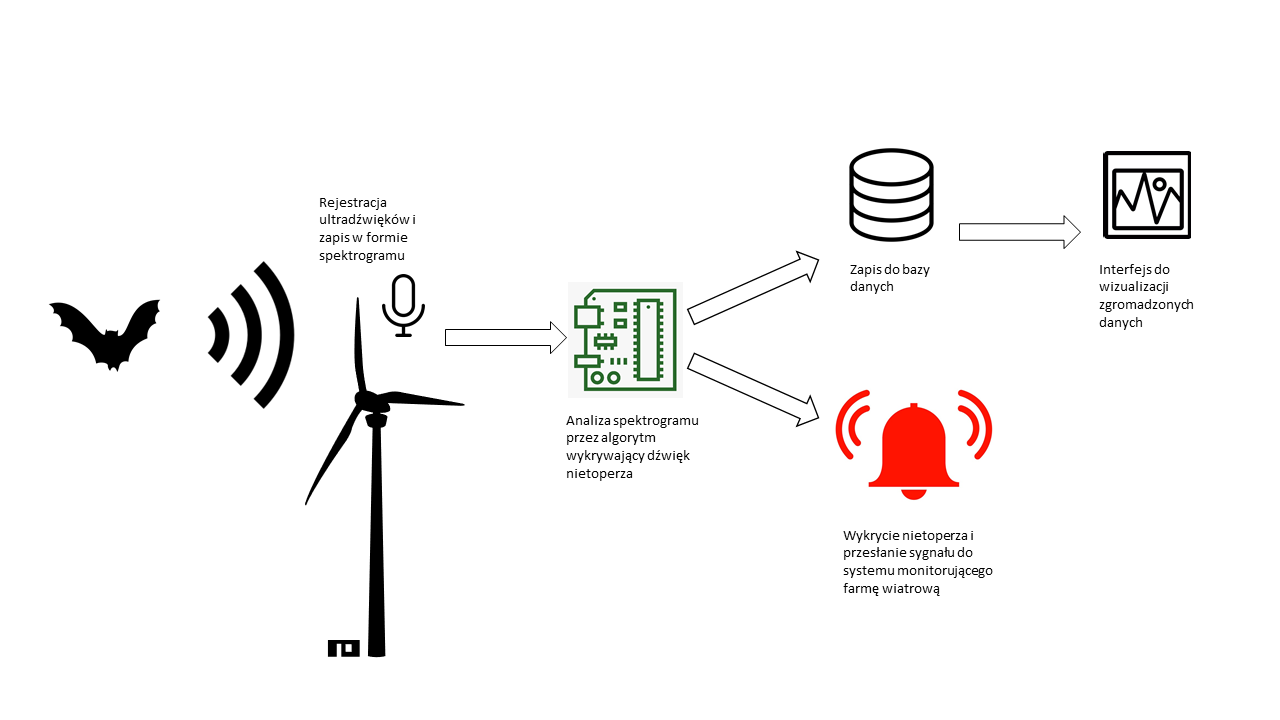
\includegraphics[width=0.8\textwidth]{sprz/rich_picture}
        \label{img:rich_picture}
    \end{figure}

  \item \textbf{Cele systemu}
  
    System ma na celu zczytywać z mikrofonu ultradźwięki wydawane przez nietoperze, przesyłać je do uprzednio wytrenowanego modelu i sygnalizować, gdy nietoperze się pojawią, podając przy tym wykryty gatunek. Jednocześnie powinien zapisywać sygnały nietoperzy w bazie danych i wizualizować je w interfejsie użytkownika.  System po dopracowaniu i ewentualnej komercjalizacji przeznaczony będzie głównie dla firm posiadających lub zarządzających dużymi farmami wiatrowymi. Korzyści wynikające z zastosowania systemu to: ograniczenie śmiertelności nietoperzy na farmach wiatrowych i możliwość zrealizowania zapisów wynikających z pozwoleń prawnych na realizację konkretnego przedsięwzięcia.

  \item \textbf{Kontekst systemu}
  
    System będzie składał się z mikrofonu ultradźwięków wraz z urządzeniem rejestrującym dźwięk (komputerem), do którego będą trafiały wszystkie nagrania, tam analizowane i wystawiające API dla systemu wyłączającego turbinę wiatrową - zamontowane na turbinie wiatrowej.

  \item \textbf{Zakres systemu (funkcjonalność)}
  
    Do głównych funkcjonalności systemu będą należały:

    \begin{itemize}
      \item Rejestracja nagrań,
      \item Przesyłanie nagrań do urządzenia wewnętrznego, na którym są one przechowywane, analizowane i wstawiane do modelu ML/DL,
      \item Analiza nagrań z udziałem modelu ML/DL pod kątem występowania nietoperzy i ich gatunków,
      \item Wizualizacja nagrań nietoperzy w bazie danych poprzez interfejs, wraz z możliwością ich szczegółowego przeglądania.
    \end{itemize}

  \item \textbf{Wymagania jakościowe i inne}
  
    System powinien spełniać następujące wymagania:

    \begin{itemize}
        \item Przenośność urządzenia zewnętrznego,
        \item Niezawodne zasilanie urządzenia zewnętrznego,
        \item Adekwatna do warunków środowiskowych i technologicznych obudowa urządzenia zewnętrznego,
        \item Niezawodność połączenia pomiędzy zewnętrznym urządzeniem rejestrującym nagrania i urządzeniem przechowującym je,
        \item Możliwość wystawienia API i wykorzystania przez system wyłączający i włączający turbinę wiatrową.
    \end{itemize}

  \item \textbf{Wizja konstrukcyjna}
  
    Urządzenie zewnętrzne będzie składało się z mikrofonu Pettersson M500-384 (i opcjonalnie z obudową) oraz urządzenia rejestrującego nagranie (np. Raspberry Pi, komputer - do ustalenia), wyposażonego w zasilanie i pamięć. Kod pobierający nagranie z mikrofonu do urządzenia rejestrującego będzie utworzony pierwotnie w Pythonie. Kod modelu ML/DL będzie napisany w Pythonie z użyciem frameworka TensorFlow, PyTorch, lub innego.  

  \item \textbf{Ograniczenia}
  
    \begin{itemize}
      \item Czas trwania projektu jest ograniczony do momentu przekazania książki dyplomowej do dziekanatu uczelni PJATK.
      \item Ograniczona dostępność nagrań głosów nietoperzy w full-spectrum – możliwa sytuacja, gdy tworzenie projektu będzie odbywało się na podstawie nagrań przetworzonych.
      \item Aktywność nietoperzy ma miejsce od końca marca do października – w związku z tym brak możliwości nagrywania ich aktywności w trakcie semestru zimowego – a tym samym brak możliwości wykonania prób hardware’u przed kwieniem 2022.
    \end{itemize}

  \item \textbf{Słownik pojęć}
  
    Nagranie full-spectrum – nagranie rejestracji ultradźwięków w pełnym wymiarze

    ML (machine learning, uczenie maszynowe) – obszar sztucznej inteligencji wykorzystujący algorytmy i modele matematyczne, które automatycznie poprawiają się poprzez ekspozycję na dane, w celu prognozowania lub podejmowania decyzji dot. nowo dostarczanych danych

    DL (deep learning) – podzbiór ML wykorzystujący tzw. sieci neuronowe, w której pojedyncze neurony tworzą warstwy i stanowią de facto mnożenie wartości wejściowych z początkowo losowo przypisanymi wagami, gdzie wyniki z poszczególnych wejść są sumowane i przekazywane do tzw. funkcji aktywacji, które decydują czy i jakie wyniki przekazać do kolejnej warstwy neuronów.

\end{enumerate}

\section{Specyfikacja wymagań systemowych}

\begin{documenttable}[]
  \projectname{Batmonit}
  \customer{Bioseco S.A.}
  \contractor{PJATK}
  \projectteam{
    \begin{enumerate}
      \item Juliusz Orłowski
      \item Jakub Prucnal
      \item Magdalena Wybraniec
    \end{enumerate}
  }
  \projectlead{
    \begin{enumerate}
      \item Dawid Gradolewski
    \end{enumerate}
  }
  \documentname{Specyfikacja Wymagań Systemowych}
  \documentowner{Jakub Prucnal}
  \projectsupervisor{dr Tadeusz Puźniakowski}
\end{documenttable}
\begin{center}
  \begin{tabular}{ |p{0.1\linewidth}|p{0.28\linewidth}|p{0.2\linewidth}|p{0.24\linewidth}|p{0.12\linewidth}| }
    \hline
    \multicolumn{5}{|c|}{\textbf{Historia dokumentu}} \\
    \hline
    \textbf{Wersja} & \textbf{Opis modyfikacji} & \textbf{Rozdział/strona} & \textbf{Autor modyfikacji} & \textbf{Data}\\
    \hline
    {1.0} & {Wstępna wersja} & {Całość} & {Jakub Prucnal} & {2021-12-05}\\
    \hline
    {2.0} & {Całość niektórych punktów, poprawki reszty} & {punkty 2, 2.1, 2.3} & {Magdalena Wybraniec} & {2021-12-19}\\
    \hline
  \end{tabular}
\end{center}

\begin{enumerate}[label=\textbf{\arabic*}.]
  \item \textbf{Wprowadzenie – o dokumencie}
    \begin{enumerate}[font=\bfseries]
      \item \textbf{Cel dokumentu}
      
        Zdefiniowanie wymagań na podstawie analizy otoczenia projektu oraz analizę potrzeb klienta.

      \item \textbf{Zakres dokumentu}
      
        Określenie udziałowców, zdefiniowanie wymagań, analiza otoczenia projektu.

      \item \textbf{Dokumenty powiązane}
      
        Karta Projektu (KP)
        Dokument Założeń Wstępnych (DZW)
        Rich Picture

      \item \textbf{Odbiorcy}
      
        \begin{itemize}
          \item Opiekun projektu Tadeusz Puźniakowski,
          \item Zespół projektowy,
          \item Przedstawiciele zleceniodawcy: Dawid Gradolewski oraz Damian Dziak
          \item Zleceniobiorca
        \end{itemize}  

      \item \textbf{Słownik pojęć}
      
        Nagranie full-spectrum – nagranie rejestracji ultradźwięków w pełnym wymiarze
        ML (machine learning, uczenie maszynowe) – obszar sztucznej inteligencji wykorzystujący algorytmy i modele matematyczne, które automatycznie poprawiają się poprzez ekspozycję na dane, w celu prognozowania lub podejmowania decyzji dot. nowo dostarczanych danych 
        DL (deep learning) – podzbiór ML wykorzystujący tzw. sieci neuronowe, w której pojedyncze neurony tworzą warstwy i stanowią de facto mnożenie wartości wejściowych z początkowo losowo przypisanymi wagami, gdzie wyniki z poszczególnych wejść są sumowane i przekazywane do tzw. funkcji aktywacji, które decydują czy i jakie wyniki przekazać do kolejnej warstwy neuronów.      

    \end{enumerate}
  \item \textbf{Projekt w kontekście}
    \begin{enumerate}[font=\bfseries]
      \item \textbf{Kontekst biznesowy}
      
        \begin{figure}[h]
          \centering
          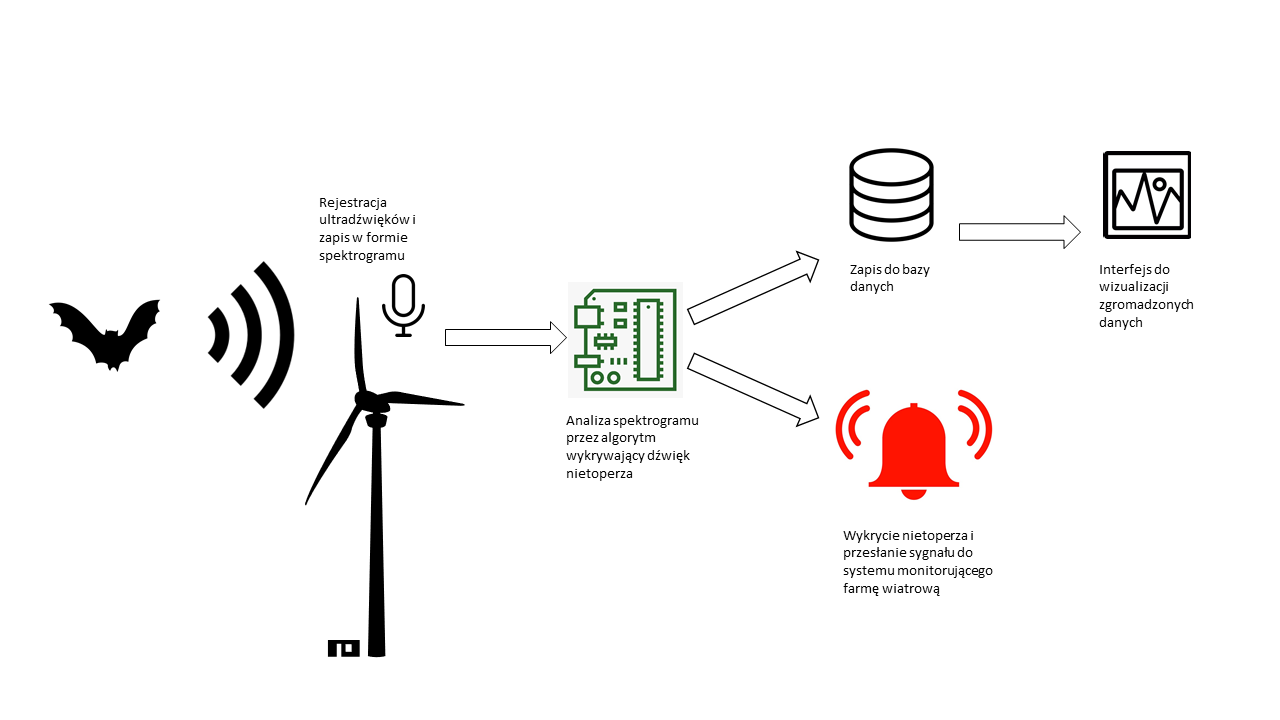
\includegraphics[width=0.8\textwidth]{sprz/rich_picture}
          \label{img:rich_picture}
        \end{figure}

      \item \textbf{Udziałowcy}
      
        \begin{stakeholder}[label={},caption={Klient}][]
          \id{UNB 01}
          \name{Klient}
          \descr{Firma Bioseco}
          \type{Nieożywiony, bezpośredni}
          \viewpoint{Techniczny, ekonomiczny, operatora systemu}
          \limitations{Brak ograniczeń, jest głównym udziałowcem}
          \requ{}
        \end{stakeholder}
        \begin{stakeholder}[label={},caption={Zespół projektowy}]
          \id{UOB 01}
          \name{Zespół projektowy}
          \descr{Zespół deweloperów, którzy tworzą projekt}
          \type{Ożywiony, bezpośredni}
          \viewpoint{Techniczny, wytwórczy}
          \limitations{Nie specyfikuje finansów}
          \requ{}
        \end{stakeholder}
        \begin{stakeholder}[label={},caption={Opiekun projektu}]
          \id{UOP 01}
          \name{Opiekun projektu}
          \descr{dr Tadeusz Puźniakowski}
          \type{Ożywiony, pośredni}
          \viewpoint{Techniczny}
          \limitations{Nie specyfikuje finansów}
          \requ{}
        \end{stakeholder}
        \begin{stakeholder}[label={},caption={Dostarczyciele nagrań nietoperzy}]
          \id{UOP 02}
          \name{Dostarczyciele nagrań nietoperzy}
          \descr{Tribio Sp. z o.o.}
          \type{Ożywiony, pośredni}
          \viewpoint{Ekonomiczny, merytoryczny}
          \limitations{Brak wpływu na aspekty techniczne oprogramowania}
          \requ{}
        \end{stakeholder}
        \begin{stakeholder}[label={},caption={Klienci klienta}]
          \id{UNP 01}
          \name{Klienci klienta}
          \descr{Klienci firmy Bioseco, którzy przesyłają zapytania o produkt do wykrywania nietoperzy}
          \type{Nieożywiony, pośredni}
          \viewpoint{Ekonomiczny, operatora systemu}
          \limitations{Brak wpływu na aspekty techniczne}
          \requ{}
        \end{stakeholder}
        \begin{stakeholder}[label={},caption={Regulacje prawne}]
          \id{UNP 02}
          \name{Regulacje prawne}
          \descr{Regulacje prawne wynikające z prawa ochrony przyrody i prawda dotyczącego ocen oddziaływania na środowisko}
          \type{Nieożywiony, pośredni}
          \viewpoint{Legislacyjny}
          \limitations{Nie specyfikuje finansów}
          \requ{}
        \end{stakeholder}
        \clearpage

      \item \textbf{Klienci}
      
        Klienci wewnętrzni:
        \begin{itemize}
          \item Dziekan
          \item Promotor
        \end{itemize}

        Klienci zewnętrzni:
        \begin{itemize}
          \item Przedstawiciele Bioseco
          \item Przedstawiciele klientów Bioseco potrzebujący urządzenia do wykrywania nietoperzy na farmach wiatrowych by sprostać wymogom prawa ochrony przyrody
          \item Firma Pettersson, producent użytego detektora, wzmacniacza i ich oprogramowania,
          \item Firma Tribio, główny dostawca nagrań nietoperzy do modelu DL
        \end{itemize}

      \item \textbf{Charakterystyka użytkowników}

        \textbf{Administrator} będzie zajmować się testowaniem systemu i zgrywaniem bazy danych uzyskanych w trakcie gdy system jest włączony. Liczebność tego użytkownika znajduje się w przedziale od 1 do 5.

        \textbf{Zwykły użytkownik} będzie zajmował się przeglądaniem i analizą danych z nagrań. Liczebność tego użytkownika znajduje się w przedziale od 1 do 20.

    \end{enumerate}

  \item \textbf{Wymagania}
  
    W niniejszym rozdziale wymienia i opisuje się wymagania narzucone przez klienta - Bioseco, przedstawicieli Uczelni – Dziekana i Promotora, a także przez aktualne standardy prawne dotyczące ochrony przyrody oraz aktualne standardy sprzętowe dotyczące nagrywania i identyfikacji nietoperzy.

    \begin{enumerate}[font=\bfseries]
      \item \textbf{Wymagania ogólne i dziedzinowe}
      
        \begin{requirementstab}[label={tab:requirements:general},caption={Baza danych nagrań głosów nietoperzy}]
          \id{WO 01}
          \priority{M}
          \name{Baza danych nagrań głosów nietoperzy}
          \descr{Zebranie lub pozyskanie bazy danych głosów nietoperzy oraz jej przygotowanie, która posłuży do stworzenia modelu rozpoznawania wystąpienia nietoperza i/lub gatunku nietoperza.}
          \sholder{UOB 01, UOP 01, UNB 01}
          \reqrelated{WO 03}
        \end{requirementstab}
        \begin{requirementstab}[label={tab:requirements:general},caption={Ekologia}]
          \id{WO 02}
          \priority{M}
          \name{Ekologia}
          \descr{System ma chronić nietoperze przed szkodliwym działaniem farm wiatrowych na ich populację}
          \sholder{UNB 01, UNP 01, UNP 02}
          \reqrelated{WO 03}
        \end{requirementstab}
        \begin{requirementstab}[label={tab:requirements:general},caption={Normy prawa}]
          \id{WO 03}
          \priority{M}
          \name{Normy prawa ochrony przyrody i prawa dotyczącego ocen oddziaływania na środowisko}
          \descr{System poprzez swoją przyszłą funkcjonalność wyłączania turbiny będzie stanowił alternatywę dla jedynego obecnie rodzaju działań minimalizujących wpływ turbin na nietoperze, czyli 3 lat monitoringu porealizacyjnego i adekwatnych do jego wyników, narzuconych z góry okresowych wyłączeń turbin, co przyniesie znaczne oszczędności dla deweloperów farm wiatrowych.}
          \sholder{UNP 02}
          \reqrelated{WO 02}
        \end{requirementstab}
        \begin{requirementstab}[label={tab:requirements:general},caption={System rozpoznawania gatunków nietoperzy}]
          \id{WO 04}
          \priority{S}
          \name{System rozpoznawania gatunków nietoperzy}
          \descr{System do rozpoznawania gatunków nietoperzy jest kosztowny, stworzenie go będzie oprogramowaniem, który przyniesie dodatkowe zyski.}
          \sholder{UOB 01, UNB01}
          \reqrelated{}
        \end{requirementstab}
        \clearpage

      \item \textbf{Wymagania funkcjonalne}
      
        \begin{requirementstab}[label={tab:requirements:func1},caption={System przygotowania i normalizacji danych}]
          \id{WF01}
          \priority{M}
          \name{System przygotowania i normalizacji danych}
          \descr{Stworzenie potrzebnych funkcji w programie do oddzielenia odstających próbek i przygotowanie bazy danych do uczenia maszynowego oraz/lub uczenia sieci neuronowych}
          \acceptcrit{Baza danych uczących model oddzielona od próbek odstających i przystosowana do zadanego zadania.}
          \inputdata{}
          \preconditions{}
          \postconditions{}
          \exceptions{}
          \implementation{}
          \sholder{UOB 01}
          \reqrelated{}
        \end{requirementstab}
        \begin{requirementstab}[label={tab:requirements:func1},caption={System rozpoznawania wystąpienia nietoperza}]
          \id{WF02}
          \priority{M}
          \name{System rozpoznawania wystąpienia nietoperza}
          \descr{Opracowanie algorytmu uczenia maszynowego oraz rozpoznawania wystąpienia nietoperza na żywo poprzez śledzenie sygnałów uzyskanych za pomocą urządzenia do detekcji.}
          \acceptcrit{Wytrenowany model do rozpoznawania wystąpienia nietoperzy.}
          \inputdata{}
          \preconditions{}
          \postconditions{}
          \exceptions{}
          \implementation{}
          \sholder{UNB 01, UNP 01}
          \reqrelated{}
        \end{requirementstab}
        \begin{requirementstab}[label={tab:requirements:func1},caption={System uczenia sieci neuronowej}]
          \id{WF03}
          \priority{C}
          \name{System uczenia sieci neuronowej}
          \descr{Opracowanie systemu do uczenia sieci neuronowej rozpoznawania gatunków nietoperzy.}
          \acceptcrit{Stworzony algorytm do tworzenia modelu do rozpoznawania gatunku nietoperza}
          \inputdata{}
          \preconditions{}
          \postconditions{}
          \exceptions{}
          \implementation{}
          \sholder{UOB 01, UOP 01}
          \reqrelated{}
        \end{requirementstab}
        \begin{requirementstab}[label={tab:requirements:func1},caption={System rozpoznawania gatunku nietoperza}]
          \id{WF04}
          \priority{S}
          \name{System rozpoznawania gatunku nietoperza}
          \descr{Opracowanie systemu do rozpoznawania gatunku nietoperza za pomocą detektora.}
          \acceptcrit{Stworzenie modelu oraz połączenie go z urządzeniem do rozpoznawania nietoperzy.}
          \inputdata{}
          \preconditions{}
          \postconditions{}
          \exceptions{}
          \implementation{}
          \sholder{UOB 01}
          \reqrelated{}
        \end{requirementstab}
        \begin{requirementstab}[label={tab:requirements:func1},caption={Interfejs do wizualizacji danych}]
          \id{WF05}
          \priority{M}
          \name{Interfejs do wizualizacji danych}
          \descr{Stworzenie interfejsu do przeglądania danych pobieranych z bazy danych i wizualizacja tych danych.}
          \acceptcrit{Stworzony interfejs działający i spełniający swoją funkcję.}
          \inputdata{}
          \preconditions{}
          \postconditions{}
          \exceptions{}
          \implementation{}
          \sholder{UOB 01}
          \reqrelated{}
        \end{requirementstab}
        \clearpage

      \item \textbf{Interfejs z otoczeniem}
      
        \begin{requirementstab}[label={tab:requirements:func1},caption={System wyłączający wiatraki}]
          \id{WF01}
          \priority{M}
          \name{System wyłączający wiatraki}
          \descr{Połączenie systemu wykrycia nietoperza z systemem wyłączającym wiatraki}
          \acceptcrit{Stworzenie punktu styku, który będzie jako output dawać sygnał do systemu wyłączającego wiatraki.}
          \inputdata{}
          \preconditions{}
          \postconditions{}
          \exceptions{}
          \implementation{}
          \sholder{UNB 01, UNP 01}
          \reqrelated{}
        \end{requirementstab}
        \begin{requirementstab}[label={tab:requirements:func1},caption={Baza danych}]
          \id{WF02}
          \priority{M}
          \name{Baza danych}
          \descr{Połączenie system z bazą danych, która będzie zbierać dane wystąpienia nietoperza}
          \acceptcrit{Stworzenie punktu styku, który będzie jako output dawać sygnał do systemu wyłączającego wiatraki.}
          \inputdata{}
          \preconditions{}
          \postconditions{}
          \exceptions{}
          \implementation{}
          \sholder{UOP 01, UNB 01}
          \reqrelated{}
        \end{requirementstab}
        \clearpage

      \item \textbf{Wymagania pozafunkcjonalne}
      


      \item \textbf{Wymagania na środowisko docelowe}
      


    \end{enumerate}

  \item \textbf{Odwołania do literatury}
\end{enumerate}
\clearpage

\section{Analiza soDIS}



\section{Diagram przypadków użycia}

\printbibliography[title={Bibliografia}, heading=bibintoc]




\end{document}
